%\documentclass[aps,prb,twocolumn,superscriptaddress,preprintnumbers,amsmath,amssymb,floatfix]{revtex4}
\documentclass[aps,prb,preprint,superscriptaddress,amsmath,amssymb,floatfix]{revtex4}
%\documentclass[aps,prl,onecolumn,groupedaddress,amsmath,amssymb,12pt]{revtex4}
\usepackage{graphicx}
\usepackage{ifthen}
\usepackage{dcolumn}% Align table columns on decimal point
\usepackage{bm}% bold math
\usepackage{multirow}
\usepackage{booktabs}
\usepackage{bm}% bold math
\usepackage{amsbsy}
\usepackage{amsmath}
\usepackage{amssymb}
\usepackage{subfigure}


%Definition of new commands
\newcommand{\f}[2]{\ensuremath{\frac{\displaystyle{#1}}{\displaystyle{#2}}}}
\newcommand{\lr}[1]{\langle{#1}\rangle}
\newcommand{\colv}[2] {\left(\begin{array}{c} #1 \\ #2 \end{array}\right)}
\renewcommand{\thefootnote}{\fnsymbol{footnote}}
\newcommand{\be} {\begin{eqnarray}}
\newcommand{\ee} {\end{eqnarray}}
%-------------------------------------------------------------------------------------------------------------------
%EQ COMMANDS
%-------------------------------------------------------------------------------------------------------------------
\newcommand{\two}{\mspace{-2.0mu}}
\newcommand{\four}{\mspace{-4.0mu}}
\newcommand{\plus}{\mspace{-4.5mu}+\mspace{-3.5mu}}
\newcommand{\minus}{\mspace{-4.5mu}-\mspace{-3.5mu}}
\newcommand{\pp}{'\mspace{-2.0mu}'}
\newcommand{\xlb}[4]{#1\ifthenelse{\equal{#2}{0}}{}{_{\alpha #2}}
\mspace{-2.0mu}\genfrac{(}{)}{0pt}{1}{\ifthenelse{\equal{#3}{0}}{0}{l #3}} {\ifthenelse{\equal{#4}{0}}{0}{b #4}}}

\newcommand{\xkv}[4]{#1\mspace{-5.0mu}\left(\mspace{-8.0mu}\begin{smallmatrix}#2\four{}\four{}\mspace{-8.0mu}&\pmb{\kappa}#3\\&\nu #4\end{smallmatrix}\mspace{-5.0mu}\right)}

\newcommand{\evect}[6]{#1\mspace{-4.0mu}\left(\mspace{-8.0mu}\begin{smallmatrix}#2\mspace{-8.0mu}&\pmb{\kappa} #3 &b #5\\&\nu #4 &\alpha #6\end{smallmatrix}\mspace{-5.0mu}\right)}

\newcommand{\varmat}[8]{\mspace{-5.0mu}\left(\mspace{-8.0mu}\begin{smallmatrix}\ifthenelse{\equal{#3}{0}}{\mspace{-8.0mu}&b_{#1}&b_{#2}\\&\alpha_{#1}&\alpha_{#2}} {\ifthenelse{\equal{#7}{0}}{#1\mspace{-8.0mu}&\pmb{\kappa}#2#3\mspace{-8.0mu}&\pmb{\kappa}#4#5\mspace{-8.0mu}&\pmb{\kappa}#6\\&\nu#2&\nu#4&\nu#6} {#1\mspace{-8.0mu}&\pmb{\kappa}#2#3\mspace{-8.0mu}&\pmb{\kappa}#4#5\mspace{-8.0mu}&\pmb{\kappa}#6#7\mspace{-8.0mu}&\pmb{\kappa}#8\\&\nu#2&\nu#4&\nu#6&\nu#8}}\end{smallmatrix}\mspace{-5.0mu}\right)}

\newcommand{\EXP}[1]{\exp\mspace{-5.0mu}\left[#1\right]\mspace{-3.0mu}}

\newcommand{\tpp}[2]{\left(\mspace{-2.0mu}\xkv{\omega}{}{}{}#1\xkv{\omega}{}{'}{'}#2\xkv{\omega}{}{\pp}{\pp}\mspace{-2.0mu}\right)}

\newcommand{\be} {\begin{eqnarray}}
\newcommand{\ee} {\end{eqnarray}}
\newcommand{\f}[2]{\ensuremath{\frac{\displaystyle{#1}}{\displaystyle{#2}}}}
\newcommand{\lr}[1]{\langle{#1}\rangle}

\newcommand{\SUM}[2]{\ifthenelse{\equal{#1}{0}}{\sum_{\alpha_{#2},b_{#2},l_{#2}}^{3,n,N}} {\ifthenelse{\equal{#1}{1}}{\sum_{\alpha_{#2},b_{#2}}^{3,n}}{\sum_{\pmb{\kappa}#2,\nu#2}^{N,3n}}}}

\newcommand{\SUMprime}[2]{\ifthenelse{\equal{#1}{0}}{\sum_{\alpha_{#2},b_{#2},l_{#2}}^{3,n,N}} {\ifthenelse{\equal{#1}{1}}{\sum_{\alpha_{#2},b_{#2}}^{3,n}}{\sum_{\pmb{\kappa}^{'}#2,\nu#2}^{N,3n}}}}

\newcommand{\SUMalpha}[2]{\ifthenelse{\equal{#1}{0}}{\sum_{\alpha_{#2}}^{3}} {\ifthenelse{\equal{#1}{1}}{\sum_{\alpha_{#2},b_{#2}}^{3,n}}{\sum_{\pmb{\kappa}#2,\nu#2}^{N,3n}}}}

\newcommand{\SUMalphap}[2]{\ifthenelse{\equal{#1}{0}}{\sum_{\alpha'_{#2}}^{3}} {\ifthenelse{\equal{#1}{1}}{\sum_{\alpha'_{#2},b'_{#2}}^{3,n}}{\sum_{\pmb{\kappa}#2,\nu#2}^{N,3n}}}}

\newcommand{\SUMb}[2]{\ifthenelse{\equal{#1}{0}}{\sum_{b_{#2}}^{n}} {\ifthenelse{\equal{#1}{1}}{\sum_{\alpha_{#2},b_{#2}}^{3,n}}{\sum_{\pmb{\kappa}#2,\nu#2}^{N,3n}}}}

\newcommand{\SUMbp}[2]{\ifthenelse{\equal{#1}{0}}{\sum_{b'_{#2}}^{n}} {\ifthenelse{\equal{#1}{1}}{\sum_{\alpha'_{#2},b'_{#2}}^{3,n}}{\sum_{\pmb{\kappa}#2,\nu#2}^{N,3n}}}}

\newcommand{\SUMl}[2]{\ifthenelse{\equal{#1}{0}}{\sum_{l_{#2}}^{N}} {\ifthenelse{\equal{#1}{1}}{\sum_{\alpha_{#2},b_{#2}}^{3,n}}{\sum_{\pmb{\kappa}#2,\nu#2}^{N,3n}}}}

\newcommand{\SUMlp}[2]{\ifthenelse{\equal{#1}{0}}{\sum_{l'_{#2}}^{N}} {\ifthenelse{\equal{#1}{1}}{\sum_{\alpha'_{#2},b'_{#2}}^{3,n}}{\sum_{\pmb{\kappa}#2,\nu#2}^{N,3n}}}}

\newcommand{\abcdt}[5]{\mspace{-4.0mu}\left(\mspace{-8.0mu}\begin{smallmatrix}&\ifthenelse{\equal{#1}{}}{a}{#1}&\ifthenelse{\equal{#3}{}}{c}{#3}\\&\ifthenelse{\equal{#2}{}}{b}{#2}&\ifthenelse{\equal{#4}{}}{d}{#4}\end{smallmatrix}\mspace{-2.0mu};\ifthenelse{\equal{#5}{}}{t}{#5}\right)}

\newcommand{\abcd}[4]{\mspace{-4.0mu}\left(\mspace{-8.0mu}\begin{smallmatrix}&\ifthenelse{\equal{#1}{}}{a}{#1}&\ifthenelse{\equal{#3}{}}{c}{#3}\\&\ifthenelse{\equal{#2}{}}{b}{#2}&\ifthenelse{\equal{#4}{}}{d}{#4}\end{smallmatrix}\mspace{-3.0mu}\right)}

\newcommand{\abt}[3]{\mspace{-4.0mu}\left(\mspace{-8.0mu}\begin{smallmatrix}&\ifthenelse{\equal{#1}{}}{a}{#1} \\&\ifthenelse{\equal{#2}{}}{b}{#2}\end{smallmatrix}\mspace{-2.0mu};\ifthenelse{\equal{#3}{}}{t}{#3}\right)}

\newcommand{\ab}[2]{\mspace{-4.0mu}\left(\mspace{-8.0mu}\begin{smallmatrix}&\ifthenelse{\equal{#1}{}}{a}{#1} \\&\ifthenelse{\equal{#2}{}}{b}{#2}\end{smallmatrix}\mspace{-3.0mu}\right)}

\newcommand{\kvbat}{\mspace{-4.0mu}\left(\mspace{-8.0mu}\begin{smallmatrix} &\pmb{\kappa} &b \\ &\nu &\alpha\end{smallmatrix}\mspace{-2.0mu};t\right)}

\newcommand{\kvbatp}{\mspace{-4.0mu}\left(\mspace{-8.0mu}\begin{smallmatrix} &\pmb{\kappa} &b' \\ &\nu &\alpha'\end{smallmatrix}\mspace{-2.0mu};t\right)}

\newcommand{\kvbaw}{\mspace{-4.0mu}\left(\mspace{-8.0mu}\begin{smallmatrix} &\pmb{\kappa} &b \\ &\nu &\alpha\end{smallmatrix}\mspace{-2.0mu};\omega\right)}

\newcommand{\kvbawp}{\mspace{-4.0mu}\left(\mspace{-8.0mu}\begin{smallmatrix} &\pmb{\kappa} &b' \\ &\nu &\alpha'\end{smallmatrix}\mspace{-2.0mu};\omega\right)}

\newcommand{\kvba}{\mspace{-4.0mu}\left(\mspace{-8.0mu}\begin{smallmatrix} &\pmb{\kappa} &b \\ &\nu &\alpha\end{smallmatrix}\mspace{-3.0mu}\right)}

\newcommand{\kvbap}{\mspace{-4.0mu}\left(\mspace{-8.0mu}\begin{smallmatrix} &\pmb{\kappa} &b' \\ &\nu &\alpha'\end{smallmatrix}\mspace{-3.0mu}\right)}

\newcommand{\kpvba}{\mspace{-4.0mu}\left(\mspace{-8.0mu}\begin{smallmatrix} &\pmb{\kappa}^{'} &b \\ &\nu &\alpha\end{smallmatrix}\mspace{-3.0mu}\right)}

\newcommand{\kva}{\mspace{-4.0mu}\left(\mspace{-8.0mu}\begin{smallmatrix} &\pmb{\kappa} \\ &\nu &\alpha\end{smallmatrix}\mspace{-3.0mu}\right)}

\newcommand{\kvap}{\mspace{-4.0mu}\left(\mspace{-8.0mu}\begin{smallmatrix} &\pmb{\kappa} \\ &\nu &\alpha'\end{smallmatrix}\mspace{-3.0mu}\right)}

\newcommand{\kvb}{\mspace{-4.0mu}\left(\mspace{-8.0mu}\begin{smallmatrix} &\pmb{\kappa} &b \\ &\nu \end{smallmatrix}\mspace{-3.0mu}\right)}

\newcommand{\kvbp}{\mspace{-4.0mu}\left(\mspace{-8.0mu}\begin{smallmatrix} &\pmb{\kappa} &b' \\ &\nu \end{smallmatrix}\mspace{-3.0mu}\right)}

\newcommand{\kvt}{\mspace{-4.0mu}\left(\mspace{-8.0mu}\begin{smallmatrix}&\pmb{\kappa} \\&\nu\end{smallmatrix}\mspace{-2.0mu};t\right)}

\newcommand{\kpvt}{\mspace{-4.0mu}\left(\mspace{-8.0mu}\begin{smallmatrix}&\pmb{\kappa}^{'} \\&\nu\end{smallmatrix}\mspace{-2.0mu};t\right)}

\newcommand{\kvw}{\mspace{-4.0mu}\left(\mspace{-8.0mu}\begin{smallmatrix}&\pmb{\kappa} \\&\nu\end{smallmatrix}\mspace{-2.0mu};\omega\right)}

\newcommand{\kv}{\mspace{-4.0mu}\left(\mspace{-8.0mu}\begin{smallmatrix}&\pmb{\kappa} \\&\nu\end{smallmatrix}\mspace{-3.0mu}\right)}

\newcommand{\kpvp}{\mspace{-4.0mu}\left(\mspace{-8.0mu}\begin{smallmatrix}&\pmb{\kappa'} \\&\nu'\end{smallmatrix}\mspace{-3.0mu}\right)}

\newcommand{\lbt}{\mspace{-4.0mu}\left(\mspace{-8.0mu}\begin{smallmatrix}&l \\&b\end{smallmatrix}\mspace{-2.0mu};t\right)}

\newcommand{\lbtp}{\mspace{-4.0mu}\left(\mspace{-8.0mu}\begin{smallmatrix}&l' \\&b'\end{smallmatrix}\mspace{-2.0mu};t\right)}

\newcommand{\lt}{\mspace{-4.0mu}\left(\mspace{-8.0mu}\begin{smallmatrix}&l\end{smallmatrix}\mspace{-2.0mu};t\right)}

\newcommand{\ltp}{\mspace{-4.0mu}\left(\mspace{-8.0mu}\begin{smallmatrix}&l'\end{smallmatrix}\mspace{-2.0mu};t\right)}

\newcommand{\lb}{\mspace{-4.0mu}\left(\mspace{-8.0mu}\begin{smallmatrix}&l \\&b\end{smallmatrix}\mspace{-3.0mu}\right)}

\newcommand{\lbp}{\mspace{-4.0mu}\left(\mspace{-8.0mu}\begin{smallmatrix}&l' \\&b'\end{smallmatrix}\mspace{-3.0mu}\right)}
%-------------------------------------------------------------------------------------------------------------------
%COMMANDS
%-------------------------------------------------------------------------------------------------------------------
\begin{document}

%\newcolumntype{d}[0]{D{!}{}{-1}}



%Title of paper
\title{Comparison and Evaluation of Spectral Energy Methods for Predicting Phonon Properties}

% repeat the \author .. \affiliation  etc. as needed
% \email, \thanks, \homepage, \altaffiliation all apply to the current
% author. Explanatory text should go in the []'s, actual e-mail
% address or url should go in the {}'s for \email and \homepage.
% Please use the appropriate macro foreach each type of information

% \affiliation command applies to all authors since the last
% \affiliation command. The \affiliation command should follow the
% other information
% \affiliation can be followed by \email, \homepage, \thanks as well.
\author{Jason M. Larkin}
\affiliation{Department of Mechanical Engineering\\Carnegie Mellon University\\Pittsburgh, PA 15213}
\author{Joseph E. Turney}
\affiliation{Department of Mechanical Engineering\\Carnegie Mellon University\\Pittsburgh, PA 15213}
\author{Alexandre D. Massicotte}
\affiliation{Department of Mechanical Engineering\\Carnegie Mellon University\\Pittsburgh, PA 15213}
\author{Cristina H. Amon}
\affiliation{Department of Mechanical Engineering\\Carnegie Mellon University\\Pittsburgh, PA 15213}
\affiliation{
Department of Mechanical \& Industrial Engineering, University of Toronto,
Toronto, Ontario, Canada M5S 3G8}
\author{A. J. H. McGaughey}
\email{mcgaughey@cmu.edu}
\affiliation{Department of Mechanical Engineering\\Carnegie Mellon University\\Pittsburgh, PA 15213}



%Collaboration name if desired (requires use of superscriptaddress
%option in \documentclass). \noaffiliation is required (may also be
%used with the \author command).
%\collaboration can be followed by \email, \homepage, \thanks as well.
%\collaboration{}
%\noaffiliation

\date{\today}

\begin{abstract}
The thermal conductivity of a dielectric or semiconducting material can be predicted using the phonon frequencies and lifetimes. Techniques for predicting these properties have been proposed based in molecular dynamics simulation, lattice dynamics calculations, and the phonon spectral energy density. Here, two expressions for the phonon spectral energy density are described and applied to three test systems: Lennard-Jones argon, Stillinger-Weber silicon, and carbon nanotubes modeled using the REBO potential. One phonon spectral energy density expression is derived from lattice dynamics theory, while the other uses only the atomic velocities from molecular dynamics simulation. We find that while the phonon spectral energy density that only uses atomic velocities can predict the phonon frequencies, it does not correctly predict the lifetimes.
\end{abstract}

% insert suggested PACS numbers in braces on next line
%\pacs{}
% insert suggested keywords - APS authors don't need to do this
%\keywords{}

%\maketitle must follow title, authors, abstract, \pacs, and \keywords
\maketitle

\clearpage
\section{\label{S-Motivation}Introduction}

eV / (Ang^2) * 1 / (

\section{\label{S-Motivation}Determining Propagating and Localized Modes}

Determine by Ioffe-Regel limit:

$\tau ~ 1/\omega$

Determine by mean free path condition:

$\Lambda \gt \lambda$

It is difficult to assign a wavevector (and hence a wavelength) to disordered mode.  Therefore, some limit must be imposed:

$\Lambda \gt a$

Where a is the lattice spacing.

\section{\label{S-Motivation}Ordered Alloys}

\subsection{\label{S-Introduction-OrderedAlloy-PhonoDispersion}Phonon Dispersion}

- $v_g(m_{r})$

- two masses with $v_g(m_{r})$, maybe compare with 4 masses with higher mass ratio.  

- Keep  $m_{avg}$ constant for all.

- run a system with a "softer" and "stiffer" LJ (smaller/bigger eps or sigma). This can be used as a comparison for the phonon/diffuson spectrums which will be shown later.  


\subsection{\label{S-Introduction-OrderedAlloy-PhonoLife}Phonon Lifetimes}

- compare lifetimes from 2 atom alloy, 4 atom alloy.  Is the reduction in thermal conductivity mostly due to the reduction in group velocities/introduction of optical modes?


\section{\label{S-Motivation}Disordered Alloys}

\subsection{\label{S-Motivation-Amorphous}Effective Phonon Dispersion}

- compare versus virtual crystal

\subsection{\label{S-Motivation-Amorphous}Effective Phonon Lifetimes}

- compare c=0.0,0.05,0.15

- why not bond disorder?  This has been investigated such as in Schelling Si/Ge \cite{schelling2002}, Marzari Si/Ge PRL \cite{Garg2011}.  Although, detailed study of PbTe/PbSe systems (Esfarjani/Shiomi preprint) demonstrate the importance of bond environment for alloys.

- if consider bond disorder, pick a "softer/stiffer" system. This system should be less/more sensitive to alloying which is discussed later.  Could reference the PbTe/PbSe paper about this.

- compare these predicted lifetimes to predictions from:

\begin{equation}\label{EQ:M:ZT}
\begin{split}
\frac{1}{\tau_{mass}} = \frac{\pi}{2N}\omega^2\kv \sum_{\pmb{\kappa'},\nu'}^{N,3n} \delta(\omega\kv - \omega\kpvp) \sum_{b}^{n}g(b)|e^*\kvba \dot e\kvba|^2 , \\
\end{split}
\end{equation}

$g(b) = \sum_{i} f_i(b)[1-m_i(b)/m_{avg}(b)]^2$

\subsection{\label{S-Motivation-Amorphous}Disappearance of SED Peaks}

- show SED plot of mode peaks from c=0.0,0.05,0.15,0.5 for any mode where a peak still shows in 0.5

\subsection{\label{S-Motivation-Amorphous}Propagating Modes in Heavily Disordered Alloys}

- Analysis of c=0.5 modes at gamma, which modes are plane-wave like? 


\section{\label{S-Motivation} Heat Transport in Amorphous System}

\subsection{\label{S-Motivation-Amorphous}Effective Phonon Dispersion}

- compare predicted sound speeds from finite dispersion acoustic branch (dk~pi/100L), bulk modulus

\subsection{\label{S-Motivation-Amorphous}Allen Feldman Diffuson Theory}

- thermal transport in terms of a diffusivity, no need for a propagation velocity

\subsection{\label{S-Motivation-Amorphous}Diffuson Lifetimes}

- measured using NMD and anharmonic MD.

- extract effective Diffuson velocity, compare to sound speed

- use sound speed to predict a phonon MFP, establish a MFP cut-off criteria to call something a phonon or not.  Could be MFP > lattice constant or something.  However, there are no wavelengths (yet).

\subsection{\label{S-Motivation-Amorphous}Propagating Modes in Amorphous System}

- Analysis of c=0.5 modes at gamma, which modes are plane-wave like? This will be the key to the length scale needed to compare with the MFP predicted above. The plane-wave like modes will be identified by fourier transforming the eigvec.  It should show content at a small number of wavevectors, and 1 should be dominant and of the order of pi/L. 

\subsection{\label{S-Motivation-Amorphous}Role of Anharmonicity in Disordered Thermal Transport}

- run harmoninc FC MD, predict thermal conductivity using GK

- compare anharmonic GK, harmonic GK, and AF predictions. May possibly need to run "stiffer" system to compare with $k_{si} = k_{ph} + k{AF} = 0.5+0.5$. 

\section{\label{S-Motivation} Thermal Diffusivity in Ordered and Disordered Systems}



- plot AF and phonon diffusivities for all systems above.  

- Show that for high mass ratio ordered alloys and disordered alloys, the thermal diffusivities are on the order of amorphous system. 

- For high mass ratio ordered alloys, it is the reduction of the group velocities through decreased acoustic and introduced optical branches. 

- For the disordered alloys, the phonon lifetimes of high frequency modes are drastically reduced as alloy concentration is increased.  Should show that this effect is less drastic for "soft" (soft bond) or "acoustically" matched systems (low mass ratio). It is more drastic for large acoustically mismatched systems (high mass ratio) or stiff systems.

- For amorphous systems, there is not a unique choice of the phonon MFP. Instead, it is helpful to consider the diffusons and their thermal diffusitivty. Compared to high mass ratio ordered alloys and heavily disordered alloys, these thermal diffusivities are comparable.  

- Compare high mass ratio ordered alloys optical branch group velocities/lifetimes (diffusivities) to amorphous diffusivities ("group velocity" and "lifetime"). Are they really distinguishable?


\subsection{\label{S-Motivation-Amorphous}Limits of the AF Diffusivity}

It was noticed by Birch and Clark (1940), and by Kit-
tel (1948) that in glasses κ(T ) at T >20K could be in-
terpreted as the specific heat C(T )/V multiplied by a
 ̄
temperature-independent diffusivity D of order a2 ωD /3
where a is an interatomic distance. In the phonon-gas
model, this would correspond to l ≈ a, too small to jus-
tify use of the model. The success of this observation
implies that the dominant normal modes in a glass are of
the D variety, not P because P implies l ≫ a, and not L
because L implies D = 0 until anharmonic corrections are
added which make D depend on T . This successful (and
we believe, essentially correct) interpretation lost favor
after Anderson localization was understood, because a
misconception arose that the P/D boundary (which cer-
tainly lies low in the spectrum of a glass) should lie close
to the E/L boundary.

Limits of D(w)

/home/jason/Downloads/papers/disorder/PhysRevB.43.6573.pdf


/home/jason/Downloads/papers/disorder/9907132.pdf

Defintions of Fourier Weights

DSF
/home/jason/Downloads/papers/disorder/PhysRevB.59.3551.pdf
Fourier Mode Weights
/home/jason/Downloads/papers/disorder/PhysRevLett.60.2280.pdf

%Understanding thermal transport in crystalline (ordered) systems requires detailed knowledge of phonons (Section \ref{S-Back-Vib-Cond}), which are the quanta of energy associated with atomic vibrations in a periodic system.\cite{dove1993,ashcroft1976,srivastava1990,wallace1972} By definition, phonons are non-localized vibrations which exist because of the translational order of the crystal. As an ordered system is disordered through the addition of defects, boundaries/interfaces, or amorphization, the vibrational modes which carry heat become localized and non-propagating and a new description is required. For completely disordered systems, such as amorphous materials, the thermal transport is modeled using completely localized vibrations (called \emph{diffusons}) which propagate diffusively (as phonons do).\cite{allen1993} However, the propagation of these diffusons is (typically) much slower than the propagation of phonons which are able to carry heat over long distances before scattering. Thus, the thermal conductivity of the amorphous phase is typically several orders of magnitude less than the crystalline phase.\cite{freeman1986,cahill1992} The first evidence of localized modes (diffusons), was reported by Keppens et al. using heat
%capacity, elastic constant and inelastic neutron-scattering
%measurements.\cite{keppens1998} 
%In general, the thermal transport in amorphous and disordered systems has contributions from localized vibrations and very-long wavelength phonon modes (see Section \ref{S-Prelim-Phonons-Amor}). Experimental measurements have shown a film thickness dependence of thermal conductivity in amorphous silicon \cite{Moon_2002} and hydrogenated amorphous silicon thin films\cite{PhysRevLett.102.035901}, which demonstrates the contribution of phonons to the thermal conductivity. Amorphous silicon/silica thin films are used in a variety of applications where managing thermal transport is important. Anomalously high measurements of thermal conductivity amorphous silicon thin films\cite{PhysRevB.81.104203} suggest that the relative contributions of ordered (phonon) and disordered vibrations to the thermal conductivity in amorphous systems requires more understanding.\cite{Zink_Pietri_Hellman_2006}
\subsection{\label{S-Motivation-Skutterudites}Thermoelectric Energy Conversion using Large Unit Cell Skutterudites}
%Thermoelectric energy generation - the transformation of waste heat into useful electricity - is a promising source of sustainable energy.\cite{ADMA:ADMA200600527} Thermoelectric materials directly convert temperature differences into electric voltage, or \emph{vice versa}, as a result of their intrinsic (atomic-level) electronic and thermal properties. Thus, thermoelectric materials can also be used in refrigeration applications. The performance of a thermoelectric device can be quantified through the dimensionless thermoelectric figure of merit,
%\begin{equation}\label{EQ:M:ZT}
%\begin{split}
%ZT = \frac{S^2\sigma T}{k_{thermal}}, \\
%\end{split}
%\end{equation}
%where $T$ is the average device temperature, $S$ is the Seebeck coefficient (the ratio of the induced thermoelectric voltage to the applied temperature difference), $\sigma$ is the electrical conductivity, and $k_{thermal}$ is the thermal conductivity. The thermal conductivity contains contributions from electrons and phonons (see Section \ref{S-Back-Vib-Cond}). 
%For thermoelectric devices to be competitive with traditional power generation cycles requires $ZT > 3$ \cite{Chen_Dresselhaus_Dresselhaus_Fleurial_Caillat_2003}. However, for waste heat retrieval any improvement in $ZT$ is desirable. Achieving this performance is challenging because the electrical and thermal properties in $ZT$ are coupled in the majority of materials \cite{ADMA:ADMA200600527,Chen_Dresselhaus_Dresselhaus_Fleurial_Caillat_2003}. The ideal thermoelectric can be thought of as an “electron-crystal/phonon-glass” (high $\sigma$, low $k_{thermal}$, see Fig. \ref{FIG:elec_crys_phonon_glass}). Reducing $k_{thermal}$ has become a primary strategy in the design of new thermoelectric materials \cite{ADMA:ADMA200600527}. Using nanostructuring to reduce $k_{thermal}$ while maintaining good electrical properties has been identified as one possible strategy \cite{B822664B}, but such materials are costly. An emerging area of study in thermoelectric power generation is the use of large unit cell (LUC) crystals \cite{nolas1999,ADMA:ADMA200600527}.
%\begin{figure}[ht]
%\centering
%\subfigure[]{
%\includegraphics[scale=0.25]{elec_crys_phonon_glass.eps}
%\label{fig:subfig1}
%}
%\subfigure[]{
%\includegraphics[scale=0.5]{skutt_rattler.eps}
%\label{fig:subfig2}
%}
%\caption[Optional caption for list of figures]{\label{FIG:elec_crys_phonon_glass} (a) LUC Skutterudites can be thought of as "electron-crystals, phonon-glass". (b) sub-unit cell effects, including the role of "rattler atoms", must be considered when characterizing the thermal transport in these LUC materials.}
%\end{figure}
%LUC crystals have an ordered (crystalline) structure, but the basic building block (unit cell) of the crystal has a large number of distinct atoms (Fig. \ref{FIG:elec_crys_phonon_glass}).\cite{cm052055b,Yang_Chen_2006,wang_232107} They are effectively disordered over length scales on the order of the atomic spacing and their thermal conductivities can be as low as a glass (amorphous material) \cite{cm052055b,Yang_Chen_2006,wang_232107}. The key advantage of LUC materials is that they are still ordered from the standpoint of electrons, making them “electron-crystal/phonon-glass” materials. Current LUC crystals have $ZT < 3$ \cite{cm052055b,Yang_Chen_2006,wang_232107} and more research is required to improve their thermoelectric performance. The LUC crystals to be studied here are Skutterudite.\cite{cm052055b} Experimental measurements of the thermoelectric properties of Skutterudites show intriguing potential,\cite{cm052055b,Yang_Chen_2006,wang_232107} but more research is required to achieve high $ZT$. 
%Current research is focused to increasing $ZT$ by reducing the $k_{thermal}$.\cite{keppens1998,Sales_Chakoumakos_Mandrus_Sharp_1999,doi:10.1021/ja063695y} The mechanisms for thermal conductivity reduction in LUC materials are still being investigated.\cite{Sales_Chakoumakos_Mandrus_Sharp_1999,qiu:063713} Some work explains the reductions in thermal conductivity in terms of a phonon picture,\cite{Toberer2011,Yang_Chen_2006,Christensen2008} while other work suggests that sub-unit cell effects are most important.\cite{PhysRevLett.82.779} It is thus difficult to develop an optimization strategy reducing the thermal transport in LUC Skutterudite materials without understanding the relative contributions of both phonons and disordered vibrational modes.
%\subsection{\label{S-Motivation-Zeolites}Large Unit Cell Zeolites for Gas Adsorption }
%\begin{figure}
%\begin{center}
%\includegraphics[scale=0.25]{alan_silica_structures.eps}
%\vspace*{-5mm}
%\end{center}
%\caption{\label{FIG:silica_structures} Silica structure building blocks and materials, incuding the LUC Zeolites. Diverse sub-unit cell structures are possible, which are likely to display unique localized vibrational properties that play an important role in thermal transport.}
%\end{figure}
%Zeolites are another class of LUC materials which are sometimes referred to as porous crystals, themselves a diverse group of materials
%characterized by large unit cells and Angstrom sized pores
%and channels.\cite{mcgaughey2004b} The size of the pores is on the same scale as the
%dimensions of atoms and molecules, leading to the use of porous crystals as molecular sieves, catalysts, and gas storage applications.\cite{dyer1988} There also is interest in the design of porous crystals with very low thermal conductivities for applications as rigid insulators and to protect stored gases from ambient temperature fluctuations which requires understanding the thermal transport properties.
%The thermal transport in zeolites and other cage-like structures is dictated by both phonons\cite{mcgaughey2004b} and localized vibrations which arise due to sub-unit cell effects.\cite{O'Keeffe20003,doi:10.1021/ar000034b} Thomas et al. used molecular simulation to show that water molecules in carbon nanotubes scatter phonons with specific vibrational frequencies related to the vibrational properites of the nanotubes and molecules \cite{thomas2010c}. The same effects are seen in molecular simulation predictions of thermal transport in carbon nanotubes on silica substrates.\cite{shiomi2011b} It is likely that adsorbed molecules in Zeolites play a similar role in scattering vibrations, but it is unclear which vibrational modes (phonons or localized) are affected.\cite{Miyamoto1994117} To design thermal properties, the mechanisms by which heat is transferred in these materials must be understood.

%\subsection{\label{S-Motivation-Hypothesis}Hypothesis}
%Based on the research provided in the above sections, the following hypothesis will be investigated in this work:
%\begin{itemize}
%\item \textit{Hypothesis: the thermal transport in amorphous and disordered materials can be accounted for using simple, computationally cheap models by considering the contribution from ordered (phonons) and disordered vibrations.}
%\item \textit{Hypothesis: understanding thermal transport in diverse LUC materials such as Skutterudites and Zeolite allotropes requires analysis of ordered (phonons) and sub-unit cell (disordered) vibrations.}
%\item \textit{Hypothesis: it is likely that the thermoelectric performance of large unit cell Skutterudites has yet to be fully realized until the ordered (phonons) and disordered contributions to minimizing thermal conductivity is understood.}
%\end{itemize}
%\clearpage
%\section{\label{S-Back}Background}
%\subsection{\label{S-Back-Vib-Cond}Vibrational Thermal Conductivity}
%Thermal conductivity in a material arises from both electronic ($k_{e}$) and vibrational
%($k_{vib}$) contributions.\cite{ashcroft1976,Slack1979} The electronic contribution is important in metals and is well described by the Wiedemann–Franz law, increasing linearly with the electrical conductivity and temperature. For dielectric and semiconducting materials, the vibrational contribution is dominant and
%\begin{equation}\label{EQ:M:k_thermal}
%\begin{split}
%k_{thermal} = k_{e} + k_{vib} \approx k_{vib}. \\
%\end{split}
%\end{equation}
%In this work, only dielectric and semiconducting materials are considered. The energy carriers of the vibrational conductivity are phonons, which are the quanta of energy associated with atomic vibrations.\cite{dove1993,ashcroft1976,srivastava1990,wallace1972} 
%The vibrational conductivity can be derived at the carrier (phonon) level by solving the Boltzmann transport equation under the relaxation time approximation.\cite{srivastava1990,ziman2001} For a crystal (ordered) system, the expression for the thermal conductivity is a sum over all phonon modes with mode specific properties,
%\begin{equation}\label{EQ:M:k_l,sum}
%\begin{split}
%k_{vib,\mathbf{n}}=&\sum_{\pmb{\kappa}} \sum_\nu c_{ph}\kv \pmb{v}^{2}_{g,\mathbf{n}}\kv \tau\kv.
%\end{split}
%\end{equation}
%
%\begin{equation}\label{EQ:M:k_l,sum}
%\begin{split}
%\mathbf{q} = - k \nabla T
%\end{split}
%\end{equation}
%
%\begin{equation}\label{EQ:M:k_l,sum}
%\begin{split}
%k_{\mathbf{n}}=&\sum_{\pmb{\kappa}} \sum_\nu c_{ph}\kv \pmb{v}^{2}_{g,\mathbf{n}}\kv \frac{\Lambda\kv}{|\pmb{v}_{g}|}.
%\end{split}
%\end{equation}
%
%Here, $\pmb{\kappa}$ are the allowed wavevectors in the system (see Section \ref{A-Allowed-Wavevectors-Ordered}), $\nu$ is the phonon polarization with vibrational frequency $\omega \kv$, $c_{ph}\kv$ is the mode specific heat, $v^{2}_{g,\mathbf{n}}\kv$ is the phonon group velocity in the direction $\mathbf{n}$, and $\tau\kv$ is the phonon lifetime. 
%The phonon lifetime can be recast as a mean free path by
%\begin{equation}\label{EQ:M:phonon_mfp}
%\begin{split}
%\Lambda\kv = |\pmb{v}_{g}| \tau\kv,
%\end{split}
%\end{equation}
%which is useful for describing the scattering of phonons over length scales that can be compared to relevant length scales in the system (see Section \ref{S-Prelim-Phonon-Scattering}).
%\subsection{\label{S-Back-Lattice-Cond-Range}Range of Vibrational Thermal Conductivity}
%The vibrational conductivity of a variety of solids (single species crystals (e.g., Si, diamond), amorphous solids ( e.g., amorphous silica and carbon), and Large Unit Cell (LUC) materials (e.g., Skutterudites, Zintl compounds)) are showin in Fig. \ref{FIG:k_thermal_solids}. Over the range of solids and temperatures, the vibrational conductivity can vary by up to $10^6$. The vibrational conductivity of LUC materials are comparable to those of the amorphous solids. The vibrational conductivity of amorphous solids is refered to as the "glass" or amorphous limit (see Section \ref{S-Motivation-Amorphous}), which usually represents the lower bound of vibrational conductivity for a system which has a crystal\\
%,cahill1992}
%The behavior of vibrational conductivity at low temperatures follows a scaling because phonons are bosons, which follow Bose-Einstein statistics.\cite{srivastava1990,stephens1971,freeman1986} Once a significant number of phonon modes become occupied (particularly at high frequency), the vibrational conductivity becomes dependent on the sample boundary size which limits the phonon mean free paths (see Section \ref{S-Prelim-Phonon-Scattering}). This boundary scattering causes a maximum in the vibrational conductivity at some temperature, above which the vibrational conductivity decreases due to increasing phonon scattering (see Section \ref{S-Prelim-Vib-Cond-Ordered}). The range of decreasing vibrational conductivity with temperature can be estimated using the Debye temperature ($T_D$) which is calculated using the debye frequency ($\omega_D$) of the system.\cite{ashcroft1976,srivastava1990}
%For amorphous and disordered materials, the vibrations in the system are not completely characterized by phonons. With the exception of very long wavelength modes, the vibrational modes are localized and do not propagate like
%phonons in a crystal (see Section \ref{S-Prelim-Alloy-Amor}). This is the reason that the vibrational conductivity of amorphous and LUC materials in Fig. \ref{FIG:k_thermal_solids} generally increase monotonically with temperature. For disordered materials, Eq$.$ \eqref{EQ:M:k_l,sum} can only describe the very low-frequency phonon-like modes which have a non-zero group velocity. However, Eq$.$ \eqref{EQ:M:k_l,sum} is still commonly used to estimate vibrational conductivity in an amorphous disordered system. Here, one typically assumes one of the following: 
%\begin{itemize}
%\item The group velocity for all the modes is
%equal to the speed of sound and the mean free path is given
%by the average interatomic distance. \cite{einstein1911,kittel1949} This is referred to as the Einstein model.
%\item The group velocity for all the modes is
%equal to the speed of sound and the lifetime (mean free path) is given
%by the inverse of the mode frequency (half the mode wavelength, see Section \ref{S-Research-Objectives-1}).\cite{cahill1992} This is referred to as the Cahill-Pohl (CP) model.
%\end{itemize}
%This approach can be used to estimate a lower limit to the vibrational conductivity in amorphous and disordered systems.\cite{cahill1987,cahill1992} However, theory\cite{allen1993}, experimental measurements\cite{PhysRevB.34.5696}, and simulation results\cite{shenogin2009} show that this approach can give only a qualitative description of the vibrations which contribute to the thermal conductivity in disordered systems (see Section \ref{S-Prelim-Alloy-Amor}).
%\begin{figure}
%\begin{center}
%\includegraphics[scale=1.0]{k.eps}
%\vspace*{-5mm}
%\end{center}
%\caption{\label{FIG:k_thermal_solids}Temperature dependence of the vibrational conductivity of a variety of solids: (single species crystals (e.g., Si, diamond), amorphous solids ( e.g., amorphous silica and carbon), and Large Unit Cell (LUC) materials (e.g., Skutterudites, Zintl compounds)). Over the range of solids and temperatures, the vibrational conductivity can vary by up to $10^6$. The vibrational conductivity of LUC materials are comparable to those of the amorphous solids. The vibrational conductivity of amorphous solids is refereed to as the "glass" or amorphous limit, which usually represents the lower bound of vibrational conductivity for a system which has a crystalline phase.\cite{cahill1987,cahill1992} }
%\end{figure}
%\clearpage
%
%\section{\label{S-Prelim}Range of Virbational Conductivity in Lennard-Jones Systems}
%
%\subsection{\label{S-Prelim-Vib-Cond-Ordered}Green-Kubo Predictions}
%
%\begin{figure}
%\begin{center}
%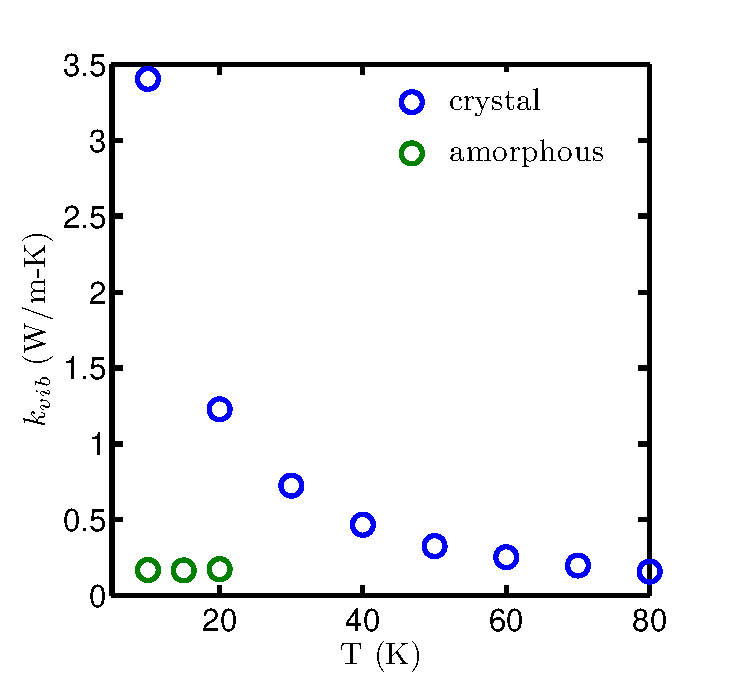
\includegraphics[scale=0.6]{LJ_amor_GK.eps}
%\vspace*{-5mm}
%\end{center}
%\caption{\label{FIG:LJ_amor_GK}The temperature dependence of crystalline and amorphous Lennard-Jones samples predicted using MD simulations and the Green-Kubo method.\cite{mcgaughey2004a} For the crystal the vibrational conductivity follows a $1/T$ scaling (consistent with the phonon-phonon lifetime scaling in Eq$.$ \eqref{EQ:M:tau_p-p}) , while the amorphous vibrational conductivity is temperature independent. Both of these trends are due to the lack quantum mechanical effects in the classical MD simulations. }
%\end{figure}
%
%\begin{figure}
%\begin{center}
%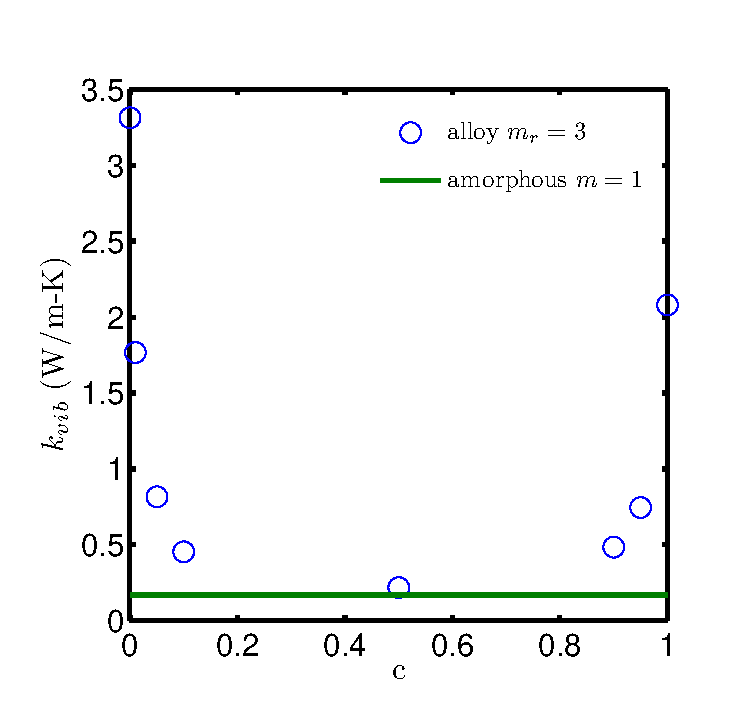
\includegraphics[scale=0.6]{LJ_alloy_GK.eps}
%\vspace*{-5mm}
%\end{center}
%\caption{\label{FIG:LJ_alloy_GK} The vibrational conductivity of LJ alloys predicted using MD simulations and the Green-Kubo method. The predicted thermal conductivities are for a LJ alloy of the form $m^a_{1-c}m^b_{c}$, where $m^a =$ 1, $m^b=$ 3, and $m_r = m^a/m^b=$ 3 (in LJ units). As the alloy concentration is increased perturbatively, the vibrational conductivity drops quickly and saturates to a minimum at $c=0.5$. For $c=0.5$ the system is heavily disordered and the vibrational conductivity approaches that of an amorphous system.}
%\end{figure}
%
%Need:
%
%GK of amorphous at m=2
%
%GK of perfect at m=2
%
%\section{\label{S-Prelim}Disordered Modes}
%
%\subsection{\label{S-Prelim-Vib-Cond-Ordered}Disordered Modes in a Crystal}
%
%Need:
%
%Understanding of:
%
%AF of perfect
%
%AF of Alloys, systems on lattice
%
%\subsection{\label{S-Prelim-Vib-Cond-Ordered}Disordered Modes in a Amorphous}
%
%
%\section{\label{S-Prelim}Preliminary Work}
%\subsection{\label{S-Prelim-Vib-Cond-Ordered}Vibrational Thermal Conductivity in Ordered Materials}
%For ordered (crystalline) systems, there are many phonon transport models which attempt to express Eq$.$ \eqref{EQ:M:k_l,sum} as an integral quantity,\cite{callaway1959,holland1963}
%\begin{equation}\label{EQ:M:k_integral}
%\begin{split}
%k_{vib}=& \int_{0}^{\omega_{max}} c(\omega)_{ph} D(\omega) D_{ph}(\omega) d\omega,
%\end{split}
%\end{equation}
%
%\begin{equation}\label{EQ:M:k_integral}
%\begin{split}
%k_{vib}=& \int_{0}^{\omega_{max}} c(\omega)_{ph} D(\omega) v^2_g(\omega)\tau(\omega) d\omega,
%\end{split}
%\end{equation}
%
%\begin{equation}\label{EQ:M:D_ph}
%\begin{split}
%D_{ph}(\omega) = v^2_g(\omega)\tau(\omega), 
%\end{split}
%\end{equation}
%
%
%\begin{equation}\label{EQ:M:k_integral}
%\begin{split}
%c(\omega)_{ph} = \frac{k_{B}x^2}{V} \frac{exp(x)}{[exp(x)-1]^2} \\
%x = \frac{\hbar\omega}{k_{B}T} \\
%c(\omega)_{ph} =\frac{k_{B}}{V} \\
%\end{split}
%\end{equation}
%
%
%whose terms are sometimes referred to as the properties of the frequency-dependent phonon spectrum. While Eq$.$ \eqref{EQ:M:k_integral} useful for examining general trends in vibrational conductivity, in a real system the phonon properties do not follow an analytical form (see $.$ \eqref{EQ:M:k_l,sum}). 
%In a harmonic crystalline system, phonon lifetimes are infinite, making the $k_{vib}$ infinite (see Appendix \ref{A-Derivation-SED}). The scattering of phonons in a pure crystal arises from phonon-phonon interactions, which arise from the anharmonicity of the interatomic potentials. The strength of the anharmonicity dictates the strength of the phonon-phonon interactions and hence the lifetime reduction.\cite{turney2008b} A simple model for the phonon-phonon scattering of acoustic mode phonons (dominant in crystalline thermal transport) is
%\begin{equation}\label{EQ:M:tau_p-p}
%\tau_{p-p} = \frac{(6 \pi^2)^{1/3} \bar m v_g v_p^2}{2 V^{1/3} \omega^2 \gamma^2 T },
%\end{equation}
%
%\begin{equation}\label{EQ:M:tau_p-p}
%\gamma(\omega_i) = - \frac{V}{\omega_i}\frac{\partial\omega_i}{\partial V} ,
%\end{equation}
%
%where $\bar m$ is the average crystal mass, $v_g$ is the acoustic branch group velocity, $v_p$ is the acoustic branch phase velocity, V is the system volume, $\omega$ is the phonon frequency, $\gamma$ is the mode dependent Gruneisen parameter, and $T$ is the temperature.\cite{callaway1959,holland1963} 
%The form of Eq$.$ \eqref{EQ:M:tau_p-p} and its parameters are able to explain several general trends:
%\begin{itemize}
%\item It is phonon-phonon scattering which is responsible for the decrease of thermal conductivity with temperatures seen in Fig. \ref{FIG:k_thermal_solids}. 
%\item The reduced vibrational conductivity of germanium compared to silicon can be explained in both in terms of the $\bar m$ (germanium has a larger density $\rho$ than silicon) and the group velocity (germanium has a smaller bulk modulus $B$, and $v_g \propto \sqrt{B/\rho}$.
%\item The decreased vibrational conductivity of systems which are highly anharmonic, such as weak covalently and Van der Waals bonded systems,\cite{costescu2004} is accounted for by the Gruneisen parameter. For a purely harmonic system, the mode specific Gruneisen parameter is zero and the phonon lifetimes are infinite.
%\end{itemize}
%
%The temperature dependence of crystalline and amorphous thermal conductivity can be investigated using Molecular Dynamics (MD) simulation and the Green-Kubo method.\cite{mcgaughey2004a} These MD simulations are classical and do not include any quantum mechanical effects (Section \ref{S-Motivation-Amorphous}). The Green-Kubo technique has been shown to accurately predict thermal transport for finite size systems.\cite{mcgaughey2004a} Here, model Lennard-Jones (LJ) crystal and amorphous samples are used to predict the thermal conductivity as a function of temperature (see Fig. 
%\ref{FIG:LJ_amor_GK}).\cite{mcgaughey2004a} For the crystal the vibrational conductivity follows a $1/T$ scaling (consistent with the phonon-phonon lifetime scaling in Eq$.$ \eqref{EQ:M:tau_p-p}) , while the amorphous vibrational conductivity is temperature independent. Both of these trends are due to the lack quantum mechanical effects in the classical MD simulations.
%The phonon-phonon scattering model Eq$.$ is typically used with the Debye approximation, which assumes linear and isotropic dispersion $\omega = v_g\kappa$ (or some variation\cite{callaway1959,holland1963}). If the dispersion is linear, the frequency dependent phonon density of states is
%\begin{equation}\label{EQ:M:debye_DOS}
%D(\omega) = A\omega^2,
%\end{equation}
%where $A$ is a constant related to the material properties.\cite{ashcroft1976} In a real system, the phonon dispersion is not linear, which can be demonstrated by calculating the density of states for a LJ crystal (Fig$.$ \ref{FIG:crys_amor_DOS}). The density of states is calculated using Lattice Dynamics (LD) calculations.\cite{dove1993} At low frequencies the density of states follows a Debye type scaling ($\omega<$15), but diverges at high frequency due non-linearity of the phonon dispersion (see Section \ref{S-Prelim-Phonon-Dispersion}). For the amorphous system, the majority of vibrations in the system are not phonons and thus the density of states only follows Debye scaling at very low frequencies (long wavelengths, see Section \ref{S-Prelim-Phonon-Dispersion}).
%\begin{figure}[ht]
%\centering
%\subfigure[]{
%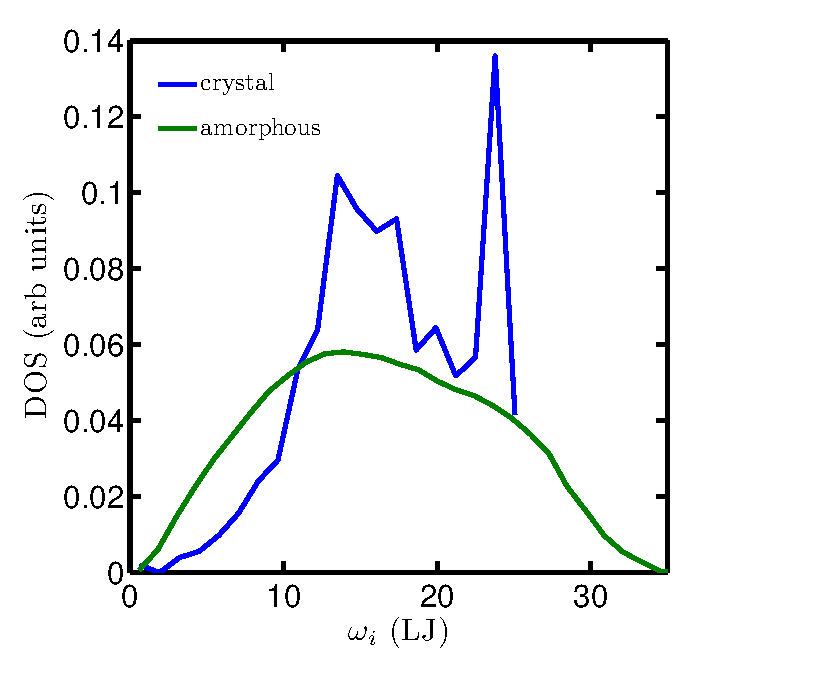
\includegraphics[scale=0.5]{LJAr_crys_amor_DOS.eps}
%\label{FIG:crys_amor_DOS}
%}
%\subfigure[]{
%\includegraphics[scale=0.5]{phonon_life_scaling.eps}
%\label{FIG:phonon_life_scaling}
%}
%\label{FIG:crys_dos_life}
%\caption{ (a) Density of states for a crystal and amorphous Lennard-Jones system (total number of atoms is 2048). For the crystal, the density of states roughly follows a Debye scaling at low frequencies ($\omega<$15), above which the density of states does not follow an analytical form due to the non-linear dispersion. For the amorphous system, the majority of vibrations in the system are not phonons and thus the density of states only follows Debye scaling at very low frequencies. (b) Phonon lifetimes as a function of frequency at T=20 K for the same Lennard-Jones crystal used to calculate the density of states in Fig. \ref{FIG:crys_amor_DOS}. The lifetimes roughly follow the scaling with frequency in Eq. \eqref{EQ:M:tau_p-p} over the same frequency interval as the Debye scaling in the density of states ($\omega<$15).}
%%\subref{fig:subfig2} and \subref{fig:subfig3}
%\end{figure}
%
%\begin{figure}
%\begin{center}
%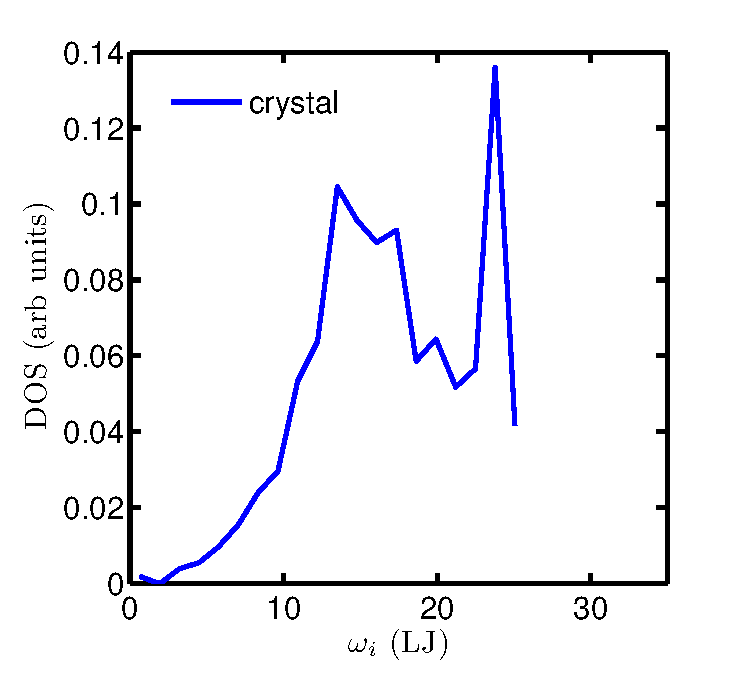
\includegraphics[scale=0.5]{LJAr_crys_DOS.eps}
%\vspace*{-5mm}
%\end{center}
%\caption{\label{FIG:LJ_amor_GK}The temperature dependence of crystalline and amorphous Lennard-Jones samples predicted using MD simulations and the Green-Kubo method.\cite{mcgaughey2004a} For the crystal the vibrational conductivity follows a $1/T$ scaling (consistent with the phonon-phonon lifetime scaling in Eq$.$ \eqref{EQ:M:tau_p-p}) , while the amorphous vibrational conductivity is temperature independent. Both of these trends are due to the lack quantum mechanical effects in the classical MD simulations. }
%\end{figure}
%
%The phonon lifetimes in a LJ crystal also do not strictly follow the lifetime scaling model in Eq$.$ \eqref{EQ:M:tau_p-p}. The phonon lifetimes for the LJ crystal are predicted using the Normal Mode Decomposition (NMD) method (Appendix \ref{A-Phonon-Life-SED}) for a system size $N_0=8$ (2048 atoms) at T=20 K. For the LJ crystal, the phonon lifetimes scale with $\omega^{-2}$ over roughly the same frequency range as the Debye scaling of the density of states, see Fig. \eqref{FIG:phonon_life_scaling}. For the predicted vibrational conductivity of this system ($k_{vib} = 1.2$ W/m-K), only 45.6$\%$ of the contribution comes from phonons which roughly follow the Debye approximation (for $\omega<$15). These considerations demonstrate the usefulness and limitations of analytical models used to replace Eq$.$ \eqref{EQ:M:k_l,sum}.
%\subsection{\label{S-Prelim-Phonon-Scattering}Phonon Scattering Mechanisms}
%The various phonon scattering mechanisms described in this section scatter phonons with varying strength across the phonon spectrum. The phonon-phonon scattering described by Eq$.$ \eqref{EQ:M:tau_p-p} scatters phonons strongly across a wide frequency range. Phonon scattering by boundaries ($\tau_{b}$) and defects ($\tau_{b}$) affect very different intervals of the frequency-dependent phonon spectrum (Eq$.$ \eqref{EQ:M:k_integral} ).
%A simple and effective model for boundary scattering is to assume diffuse scattering, which for the case of a thin film (Fig. \ref{FIG:phonon_scattering_diag}) gives
%\begin{equation}\label{EQ:M:tau_b}
%\tau_{b} = L/v_g.
%\end{equation}
%When the phonon mean free path is greater than the film thickness, it's mean free path is limited by this length scale. The concept can be extended to nanostructures of arbitrary geometry.\cite{mcgaughey:061911} This boundary scattering model can account for several effects:
%\begin{itemize}
%\item It is boundary scattering which is dominant and responsible for slowing the rate of vibrational conductivity increase at low temperatures in Fig$.$ \ref{FIG:k_thermal_solids}.
%\item Boundary scattering describes the decrease in vibrational conductivity in thin films of decreasing thickness and other nanostructures of various decreasing system geometries.\cite{mcgaughey:061911}
%\end{itemize}
%\begin{figure}
%\begin{center}
%\includegraphics[scale=0.25]{phonon_scattering_diagram.eps}
%\vspace*{-5mm}
%\end{center}
%\caption{\label{FIG:phonon_scattering_diag} The various phonon scattering mechanisms scatter phonons with varying strength across the frequency spectrum. The phonon-phonon scattering is intrinsic and exists even in perfect crystals. Boundary scattering is responsible for decreasing the long lifetimes (mean free paths) of low frequency phonons which carry a significant amount of heat. Defect scattering is of Rayleigh type, where high frequency modes are scattered most strongly.}
%\end{figure}
%Boundary scattering is responsible for decreasing the long lifetimes (mean free paths) of low frequency phonons which carry a significant amount of heat, making it particularly effective at decreasing the thermal conductivity of systems with length scale of 100s of $\mu$m and less.\cite{mcgaughey:061911}
%Defect scattering in the form of atomic mass and/or size variation can be modeled assuming the defects are a perturbation, by
%\begin{equation}\label{EQ:M:tau_d}
%\frac{1}{\tau_{d}} = \frac{V \omega^4}{4 \pi v_p^2 v_g} ( \sum_i c_i(1-m_i/\bar m)^2 + \sum_i c_i(1-r_i/\bar r)^2 ),
%\end{equation}
%where $c_i$ is the fraction, $m_i$ is the mass, and $r_i$ is the radius of species i and $\bar r$ is the average atomic radius.\cite{klemens1955,klemens1957} The frequency dependence is the same as Rayleigh scattering, where high frequency modes are scattered most strongly. 
%\subsection{\label{S-Prelim-Dilute-Alloys}Dilute Alloys}
%
%\begin{equation}\label{EQ:M:tau_matthiessen}
%\frac{1}{\Lambda} = \frac{1}{\Lambda_{p-p}} + \frac{1}{\Lambda_{b}} ,
%\end{equation}
%
%\begin{equation}\label{EQ:M:tau_matthiessen}
%\begin{split}
%\hat{H}\Psi = [\hat{T} + \hat{V}_{Har} + \hat{V}_{ext} + \hat{V}_{xc}]\Psi ,
%\end{split}
%\end{equation}
%
%\begin{equation}\label{EQ:M:tau_matthiessen}
%\begin{split}
%n(\mathbf{r}) = \Psi^* \Psi ,
%\end{split}
%\end{equation}
%
%
%Experimental measurements\cite{PhysRevB.71.235202} and atomistic simulation predictions\cite{shiomi2011a} show phonons still dominate the thermal transport in weakly perturbed systems such as dilute alloys.\cite{callaway1959} The reduction in phonon lifetimes can be accounted for using Matthiessen's rule,
%\begin{equation}\label{EQ:M:tau_matthiessen}
%\frac{1}{\tau} = \frac{1}{\tau_{p-p}} + \frac{1}{\tau_{b}} + \frac{1}{\tau_{d}},
%\end{equation}
%where $\tau_{p-p}$ accounts for phonon-phonon scattering, $\tau_{b}$ accounts for boundary scattering, $\tau_{d}$ accounts for defect scattering. These scattering mechanisms can be understood by considering the phonon mean free path $\Lambda\kv$ and the illustration in Fig$.$ \ref{FIG:phonon_scattering_diag}.
%The vibrational conductivity of LJ alloys can be predicted using MD simulations and the Green-Kubo method (Fig. \ref{FIG:LJ_alloy_GK}). The predicted thermal conductivities are for a LJ alloy of the form $m^a_{1-c}m^b_{c}$, where $m^a =$ 1, $m^b=$ 3, and $m_r = m^a/m^b=$ 3 (in LJ units). As the alloy concentration is increased perturbatively, the vibrational conductivity drops quickly and saturates to a minimum at $c=0.5$. For $c=0.5$ the system is heavily disordered and the vibrational conductivity approaches that of an amorphous system.
%\subsection{\label{S-Prelim-Alloy-Amor}High Concentration Alloys and Glasses}
%The models for phonon scattering mechanisms described in Section \ref{S-Prelim-Phonon-Scattering} are successful for dilute alloys ($c<0.1$).\cite{klemens1955,klemens1957} However, as the alloy concentration is increased, the vibrational modes become localized and non-propagating and a new description of the vibrational modes which carry the heat is required. For even more disordered systems, such as amorphous materials, the thermal transport is modeled using completely localized vibrations (called \emph{diffusons}) which propagate diffusively, as phonons do.\cite{allen1993} However, the propagation of these diffusons is (typically) much slower than the propagation of phonons which are able to carry heat over long distances before scattering. Thus, the vibrational conductivity of amorphous phase is typically several orders of magnitude less than crystalline phase.\cite{freeman1986,cahill1992}
%The diffuson theory of Allen and Feldman is different than the phenomenological models discussed in Section \ref{S-Motivation-Amorphous} in that the only allowed wavevector is strictly $\mathbf{\kappa}= 0$ since the system is disordered. In reality, the vibrational conductivity has contributions from very-long wavelength phonon-like modes (see Section \ref{S-Prelim-Phonon-Scattering}). The disordered contribution to vibrational conductivity, $k_{AF}$, is given by
%\begin{equation}\label{EQ:M:k_AF}
%k_{AF} = \sum_i C(\omega_i) D_{AF}(\omega_i)
%\end{equation}
%where $C(\omega_i)$ and $D_{AF}(\omega_i)$ are the diffuson mode specific heat and diffusivity. The vibrational conductivity at low temperatures in disordered and amorphous materials is due to the low temperature behavior of the specific heat $C(\omega_i)$, which is dictated by Bose-Einstein statistics.\cite{allen1993} The theory of Allen and Feldman is purely harmonic. In the classical harmonic limit, $C(\omega_i) = k_{B}$ and $k_{AF}$ is temperature independent, which can be used to understand the amorphous LJ temperature independence of vibrational conductivity in Section \ref{S-Prelim-Vib-Cond-Ordered}.
%\begin{figure}
%\begin{center}
%\includegraphics[scale=0.6]{phonon_diff.eps}
%\vspace*{-5mm}
%\end{center}
%\caption{\label{FIG:phonon_diff} plot comparison of phonon diffusivity versus AF mode diffusivity for a 256 atom LJ crystal and amorphous system. For both systems, the total number of vibrational modes is the same.}
%\end{figure}
%Taking the phonon mode specific heat to be $c_{ph} \kv = k_{B}$, the phonon mode specific vibrational conductivity (Eq$.$ \eqref{EQ:M:k_l,sum}) can be written as
%\begin{equation}\label{EQ:k_sum}
%\begin{split}
%k_{vib,\mathbf{n}}=&\sum_{\pmb{\kappa}} \sum_\nu k_{B} D_{ph}\kv,
%\end{split}
%\end{equation}
%and the vibrational conductivity is determined by the phonon mode diffusitivies, defined as
%\begin{equation}\label{EQ:k_sum}
%\begin{split}
%D_{ph}\kv = v\kv^{2} \tau\kv.
%\end{split}
%\end{equation}
%This concept is useful for understanding how the relevant phonon properties (lifetime and group velocity) affect the thermal transport. It is also useful for comparing the relative transport strength of diffusons and phonons. Fig. \ref{FIG:phonon_diff} plots the phonon and diffuson mode diffusivities of a 256 atom LJ crystal and amorphous system at T = 20 K. The number of vibrational modes is the same for these two systems, but the relative magnitudes of the diffusivities vary greatly. The phonons diffusivities are generally greater than the diffuson diffusivities. However, Brioullin zone boundary (see Section \ref{A-Allowed-Wavevectors-Ordered}) phonon modes have a finite lifetime but vanishing group velocities, giving $D_{ph}\kv = 0$.\cite{dove1993} For crystalline systems with many atoms in the unit cell, the presence of optical phonon modes begins to trap heat in low-group velocity branches ($D_{ph}\kv \approx 0$, see Section \ref{S-Prelim-Phonon-Dispersion}), making the distinction between phonons and diffusons diffuclt. Based on their contribution to vibrational conductivity, these low diffusivity optical phonons are thermally indistinguishable from diffusons.
%The parameters defining the phonon diffusivity (phonon lifetime and group velocity) are generally well-understood. In particular, design strategies to minimize both of these parameters exist (see Sections \ref{S-Prelim-Phonon-Scattering} and \ref{S-Prelim-Phonon-Dispersion} ). However, the design strategies to control the diffusons diffusivities ($D_{AF}$) are not well understood.\cite{allen1993,shenogin2009} The diffuson theory does not consider the effects of anharmonicity, which cane be investigated using a combination of MD simulations and LD calculations.\cite{shenogin2009}
%\subsection{\label{S-Prelim-Phonon-Dispersion}Importance of Phonon Dispersion}
%\begin{figure}
%\begin{center}
%\includegraphics[scale=0.6]{GULP_disp_mass_ratio.eps}
%\vspace*{-5mm}
%\end{center}
%\caption{\label{FIG:crys_disp_mass_ratio} Dispersion plots for Lennard-Jones systems with varying number of atoms in the unit cell ($b=1..4$) and mass ratio ($m_r$) for wavevectors in the direction $2\pi/a[1 0 0]$. (a) Dispersion plot using the FCC primitive unit cell ($b=1$), which shows that only acoustic phonon branches exist in the system. The edge of the Brillouin zone in this direction is $2\pi/a[1 0 0]$. (b) Dispersion plot using the cubic conventional unit cell ($b=4$), where every atom in the unit cell is identical ($m_r=1$). Compared to the primitive cell, the Brillouin zone edge is at $\pi/a[1 0 0]$ where the acoustic branches have been "folded in".\cite{turneythesis} Other than these considerations, the choice of unit cell for the single species system does not affect the dispersion. (c) System with two unique atom types in the conventional unit cell with a mass ratio $m_r=3$, which creates optical branches with low group velocity and reduced group velocity acoustic branches. (d) System with $b=4$ unique atoms types in the unit cell with high mass ratio ($m_r=12$), which increases the number of optical branches and further reduces the acoustic group velocities. }
%\end{figure}
%\begin{figure}
%\begin{center}
%\includegraphics[scale=0.6]{amor_disp.eps}
%\vspace*{-5mm}
%\end{center}
%\caption{\label{FIG:amor_phonon_disp} Dispersion of a 256 atom amorphous Lennard-Jones solid with simulation cell size $L=4a$, where $a$ is the FCC crystal lattice constant of the LJ system. The phonon-like acoustic group velocity (sound speed) can be detected at small but finite wavevector. The vast majority of modes in the system are localized vibrations (diffusons) which appear as optical branches with nearly zero group velocity.}
%\end{figure}
%Real phonon dispersion in crystalline systems is non-linear. For single mass species LJ crystal, the choice of unit cell is will dictate the allowed wavevectors (see Section \ref{A-Allowed-Wavevectors-Ordered}) and hence the phonon dispersion. Dispersion plots for the primitive ($b=1$) and cubic conventional ($b=4$) LJ FCC unit cells for wavevectors in the $2\pi/a[100]$ direction are shown in Fig. \ref{FIG:crys_disp_mass_ratio} (a) and (b). For the primitive and cubic conventional unit cells, the Brioullin zone boundary in this direction is defined by $2\pi/a$ and $\pi/a$. For Fig. \ref{FIG:crys_disp_mass_ratio} (c) and (d), the conventional cubic unit cell contains two (c) and four (d) unique atoms with varying mass, the largest mass ratio labeled as $m_r$. Increasing the mass ratio $m_r$ of the species in the unit cell increases the gap between optical and acoustic branches and decreases the acoustic group velocities. The Debye model (assumption of linear dispersion) largely overestimates the vibrational conductivity of high mass ratio (e.g. BaO) unit cells because of these reductions in group velocity.\cite{Toberer2011} The effect of group velocity reduction is particularly effective in reducing vibrational conductivity because the phonon diffusivities are proportional to $v^2_g$ (see Section \ref{S-Prelim-Phonon-Dispersion}).
%Phonon dispersion in multi-atom unit cell crystals contains optical phonon branches, which have low group velocity and thus contribute little to vibrational conductivity (see Section \ref{S-Prelim-Phonon-Dispersion}). More optical branches can be introduced by "zone-folding", caused by increasing the number of atoms in the unit cell (Fig. \ref{FIG:crys_disp_mass_ratio}). Zone-folding traps heat in $b-1$ optical branches and decreases the acoustic mode group velocities.\cite{PhysRev.141.767} 
%For an amorphous material (see Section \ref{S-Prelim-Phonon-Dispersion}), this folding trend is continued until nearly all of the vibrational modes in the system are trapped in optical branches with virtually zero group velocity (Fig. \ref{FIG:amor_phonon_disp}). 
%In the amorphous limit ($b=\infty$), the zone-folding effect would suggest that the heat is transported solely in optical modes as the acoustic phonon contribution goes to zero. In reality, thermal transport in amorphous materials has contributions from phonons and localized vibrations (see Section \ref{S-Motivation-Amorphous}). The presence of acoustic phonon-like modes in amorphous materials can be demonstrated by considering an amorphous system of finite size. Fig. \ref{FIG:amor_phonon_disp} shows the dispersion of a 256 atom amorphous Lennard-Jones solid with simulation cell size $L=4a$, where $a$ is the FCC crystal lattice constant of the LJ system. Since periodic boundary conditions are used, the simulation cell is the unit cell with lattice constant $L=4a$. In this sense the amorphous LJ sample is a large unit cell material. 
%By considering small but finite wavevectors in the direction $\pi/L[1 0 0]$, the sound speed (acoustic group velocity) can be detected by the presence of a single acoustic type branch (vanishing frequency at $\kappa=[0 0 0]$). The rest of the vibrational modes in the system are trapped in optical modes with virtually zero group velocity. The lowest finite frequency modes at $\kappa=[0 0 0]$ are the phonon like modes which can be supported within the amorphous large unit cell.\cite{allen1993,PhysRevE.81.021301} The rest of the finite frequency modes at $\kappa=[0 0 0]$ are the diffusons, which are non-propagating localized vibrations (see Section \ref{S-Prelim-Alloy-Amor}). 
%%\begin{figure}
%%\begin{center}
%%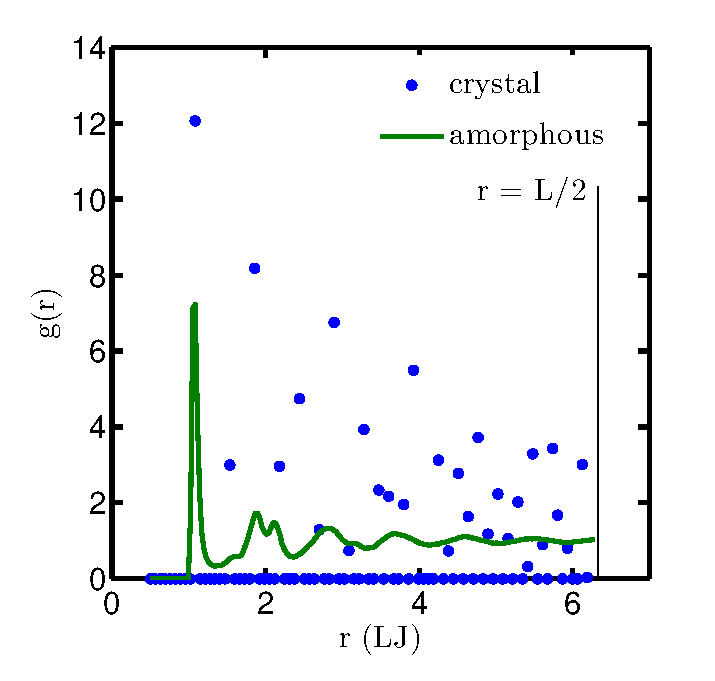
\includegraphics[angle=0,width=70.0mm]{LJAr_crys_amor_rdf.eps}
%%\vspace*{-5mm}
%%\end{center}
%%\caption{\label{FIG:crys_amor_rdf} .}
%%\end{figure}
%\subsection{\label{S-Prelim-Phonons-Amor} Phonons in Amorphous Materials }
%The diffuson theory is different than the phenomenological models discussed in Section \ref{S-Motivation-Amorphous} in that the only allowed wavevector is strictly $\mathbf{\kappa}= 0$ since the system is disordered. In reality, the vibrational conductivity has contributions from very-long wavelength phonon-like modes. Accordingly, the total vibrational conductivity in a disordered or amorphous system is the sum of contributions from diffusons and phonons,
%\begin{equation}\label{EQ:M:k_thermal}
%k_{vib} = k_{AF} + k_{ph}.
%\end{equation}
%Using the Green-Kubo method (see Section \ref{S-Prelim-Vib-Cond-Ordered}), the total vibrational conductivity of amorphous Lennard-Jones argon has been predicted to be $k_{vib}=0.17 \pm 0.1$ W/m-K. The diffuson contribution is predicted to be $k_{AF} = 0.14 \pm 0.01$ W/m-K, which suggests $k_{ph} = 0.03$ W/m-K. Similar atomistic predictions have been made for amorphous silicon, where the phonon contribution was shown to be $k_{ph} = 0.5k_{vib}$.\cite{He2011a} However, the definition of the allowed wavevectors, and hence the phonon properties of the amorphous system, is not well understood.\cite{He2011a}
%\clearpage
%\section{\label{S-Propsed-Work}Proposed Work}
%The preliminary research and work discussed in Sections \ref{S-Motivation}, \ref{S-Back}, and \ref{S-Prelim} will inform the proposed work discussed in the following sections. In particular, the hypothesis presented in Section \ref{S-Motivation} will motivate the outcomes of this work.
%\subsection{\label{S-Research-Objectives-1}Quantify Thermal Transport in Amorphous and Disordered Materials}
%\textit{Hypothesis: the thermal transport in amorphous and disordered materials can be accounted for using simple, computationally cheap models by considering the contribution from ordered (phonons) and disordered vibrations.}
%Thermal transport in crystals, alloys, and amorphous samples using model LJ systems will be studied to quantify and characterize the ordered and disordered contributions to lattice thermal conductivity. In particular, a more rigorous way to classify vibrational modes in disordered alloys and amorphous samples as phonon-like or diffuson will be investigated. These results will be compared to the phenomenological Einstein and Cahill-Pohl models,\cite{einstein1911,kittel1949,cahill1992} which assume phonon-like properties for the disordered vibrational modes. In the Cahill-Pohl model,\cite{PhysRevB.46.6131} the group velocity of all the vibrational modes is assumed to be the sound speed,
%\begin{equation}\label{E-Seq}
%v_g = v_s \propto \sqrt{B_{glass}/\rho},
%\end{equation}
%and the phonon mean free paths scale with the wavelength of the mode,
%\begin{equation}\label{EQ:M:l_glass}
%\Lambda_{glass} = \lambda /2.
%\end{equation}
%It is unclear what meaning a wavelength has for of the diffuson vibrational modes. 
%Given experimental measurements\cite{Moon_2002,PhysRevLett.102.035901,PhysRevB.81.104203,Zink_Pietri_Hellman_2006} and atomistic predictions,\cite{shenogin2009,He2011a} it is more likely that the phonon-like modes in disordered materials follow simple Debye-type scalings of their properties ( Sections \ref{S-Prelim-Vib-Cond-Ordered} and \ref{S-Prelim-Phonon-Dispersion}). This presents the opportunity of modeling thermal transport in disordered and amorphous materials using simple scaling models and diffuson theory, both of which are computationally inexpensive compared to more complicated thermal transport models.\cite{turney2008b}
%It is also unclear how to properly define the allowed wavevectors in an amorphous or disordered system (see Appendix \ref{A-Allowed-Wavevectors-Ordered}). Because of this, the way phonons interact with diffusons in these systems is not understood and will be investigated. Selection rules which determine allowed phonon-phonon interactions are based on two conservation rules. First, conservation of crystal momentum dictates that the wavevectors of the phonons involved in a 3-phonon process satisfy
%\begin{equation}\label{EQ:M:conservation-crys-mom}
%\pmb{\kappa} + \pmb{\kappa}'' = \pmb{\kappa}'' + \pmb{G}
%\end{equation}
%where $\pmb{G}$ is a reciprocal lattice vector.\cite{wallace1972,dove1993} Second, the frequencies (energies) of the phonons invovled in the scattering process satisfy\cite{wallace1972,dove1993}
%\begin{equation}\label{EQ:M:conservation-phonon-energy}.
%\omega\kv + \omega\kvp = \omega\kvpp 
%\end{equation}
%Given these conservation rules, it is unclear how the phonons which exist in amorphous and disordered materials interact with other phonons and disordered diffuson modes.
%The Allen Feldman diffuson theory is a purely harmonic one, while the MD simulations performed in this work include the full anharmonicity of the LJ interatomic potential. The effect of anharmonicity will be investigated to determine what contribution it makes to thermal transport in disordered systems using LD calculations and MD simulations. Using the information gathered from the LJ calculations, \emph{ab initio} (from first-principles)\cite{baroni2001} calculations will be designed for real amorphous systems, such as amorphous silicon. \emph{Ab initio} are computationally-intensive, but have high accuracy and predictive capability.\cite{baroni2001} 
%\subsubsection{\label{S:Resarch-Objectives-1-outcomes}Outcomes}
%The outcomes of this work will be:
%\begin{itemize}
%\item to develop methodology to identify relative contribution to thermal transport from phonons and diffusons in disordered LJ systems. 
%\item to investigate the role of anharmonicity to thermal transport in disordered systems, which can determine if computationally cheap methods and models can make accurate predictions.
%\item to design and perform \emph{ab initio} calculations to predict the thermal properties of real disordered systems such as amorphous silicon.
%\end{itemize}
%\subsection{\label{S-Research-Objectives-2}Investigate Thermal Transport in LUC Zeolites and Skutterudites}
%\textit{Hypothesis: understanding thermal transport in diverse LUC materials such as Skutterudites and Zeolite allotropes requires analysis of ordered (phonons) and sub-unit cell (disordered) vibrations, which are likely to be localized.}
%The thermal transport in Zeolites and other cage-like structures is dictated by both phonons\cite{mcgaughey2004b} and localized vibrations which arise due to sub-unit cell effects.\cite{O'Keeffe20003,doi:10.1021/ar000034b} Diverse sub-unit cell structures are possible, which are likely to display unique localized vibrational properties that play an important role in thermal transport. For gas adsorption applications, the role of scattering is not understood. Thomas et al. used molecular simulation to show that water molecules in carbon nanotubes scatter phonons with specific vibrational frequencies related to the vibrational properties of the nanotubes and molecules \cite{thomas2010c}. The same effects are seen in molecular simulation predictions of thermal transport in carbon nanotubes on silica substrates.\cite{shiomi2011b} It is likely that adsorbed molecules in Zeolites play a similar role in scattering vibrations, but it is unclear which vibrational modes (phonons or localized) are affected.\cite{Miyamoto1994117}
%Thermal transport in Zeolite structures will be investigated using LD calculations and classical MD simulations. Classical interatomic potentials exist which can describe the various Zeolite allotropes.\cite{mcgaughey2004b} Sub-unit cell effects of thermal transport will be investigated in the these diverse structures where unique bonding environments and cage-like structures likely play an important role.
%\textit{Hypothesis: it is likely that the thermoelectric performance of large unit cell Skutterudites has yet to be fully realized and requires understanding the ordered (phonons) and disordered contributions to the thermal transport to minimize thermal conductivity.}
%For many LUC materials, such as Skutterudites, two scalings of the vibrational conductivity
%(labled in Fig. \ref{FIG:snyder-kl} as $\kappa_{L}$) are shown for experimental measurements.\cite{Toberer2011} The vibrational thermal conductivity can be predicted using the Debye model (labled in Fig. \ref{FIG:snyder-kl} as $\kappa_{U}$), which predicts two
%scalings of $\kappa_{L}$ with number of atoms in the unit cell $b$. The two scalings, $b^{-1/3},b^{-1}$ are based on phonon-phonon or boundary dominant scattering.\cite{Toberer2011} The disagreement between the Debye model predictions and experimental measurements suggest the importance of the non-linear (non-Debye) dispersion (see Section \ref{S-Prelim-Phonon-Dispersion}) and sub-unit cell effects in determining the minimized vibrational conductivity in LUC materials.
%\begin{figure}
%\begin{center}
%\includegraphics[angle=0,width=70.0mm]{snyder_kl_ku-1.eps}
%\vspace*{-5mm}
%\end{center}
%\caption{\label{FIG:snyder-kl} For many LUC materials, such as Skutterudites, two scalings of the vibrational conductivity
%(labled $\kappa_{L}$) are shown for experimental measurements.\cite{Toberer2011} The vibrational thermal conductivity can be predicted using the Debye model (labled as $\kappa_{U}$), which predicts two
%scalings of $\kappa_{L}$ with number of atoms in the unit cell $b$. The two scalings, $b^{-1/3},b^{-1}$, are based on phonon-phonon or boundary dominant scattering.\cite{Toberer2011} The disagreement between the Debye model predictions and experimental measurements suggest the importance of the non-linear (non-Debye) dispersion (see Section \ref{S-Prelim-Phonon-Dispersion}) and sub-unit cell effects in determining the minimized vibrational conductivity in LUC materials.}
%\end{figure}
%Much of the excitement surrounding Skutterudites has been
%focused on the prediction and observation of a phenomena termed "rattling", observed when the guest atom
%is under-constrained and weakly bound (see Fig. \ref{FIG:elec_crys_phonon_glass}).\cite{keppens1998,Sales_Chakoumakos_Mandrus_Sharp_1999,doi:10.1021/ja063695y} Experimentally, materials in which guest atoms are strong rattlers are found to exhibit extremely low $k_{vib}$.\cite{Sales_Chakoumakos_Mandrus_Sharp_1999,qiu:063713} While it is widely accepted that rattling atoms result in strongly localized modes, the mechanism by which rattler modes reduce $k_{vib}$ is under debate. The reduction in $k_{vib}$ has been attributed to resonant scattering by the guest atom.\cite{PhysRevLett.82.779} However, the impact of rattling on the group velocity has recently been recognized as an alternative explanation of the low experimental $k_{vib}$ (see Section \ref{S-Prelim-Phonon-Dispersion}).\cite{Yang_Chen_2006,Christensen2008}
%Thermal transport in LUC Skutterudites will be investigated using a combination of LD calculations MD simulations. Several classical interatomic potentials exist which can be used to study general trends.\cite{PhysRevB.82.195207,PhysRevB.81.134301} Ultimately, \emph{ab initio} calculations will be designed for real Skutterudite systems.
%\subsubsection{\label{S:Resarch-Objectives-2-outcomes}Outcomes}
%The outcomes of this work will be:
%\begin{itemize}
%\item to characterize sub-unit cell effects such as gas adsorption in Zeolites and rattling modes in Skutterudites.
%\item to identify design strategies to manage thermal conductivity in Zeolites and reduce the thermal conductivity in Skutterudites for thermoelectric conversion applications.
%\end{itemize}
%\clearpage
%\section{\label{S-schedule}Outcomes and schedule}
%%The outcomes of this proposed research will be:
%%
%%\begin{itemize}
%%
%%\item Characterization of Thermal Transport in Disordered Materials using LJ Models
%%
%%\item Investigation of Thermal Transport in Large Unit Cell Materials
%%
%%\item Investigation of Harmonic and Anharmonic Contributions to Thermal Transport in Disordered Materials
%%
%%\item Computational Cost Analysis of Harmonic and Anharmonic Calculations
%%
%%\item Detailed Computational Framework
%%
%%
%%\end{itemize}
%The schedule for my proposed research is:
%
%\vspace*{5mm}
%\begin{tabular}{l*{6}{c}r}
%Task & Fall 2011 & Winter 2012 & Spring 2012 \\
%\hline
%Characterization of Disordered LJ Models & --------- & --------- & \\
%\hline
%Investigate (an)Harmonic Contributions & & & --------- \\
%\hline
%Task & Summer 2012 & Fall 2012 & Winter 2013 \\
%\hline
%Investigate Transport in Amorphous & --------- & --------- & \\
%Si using Ab-Initio Calculations \\
%\hline
%Investigate Transport in & & & --------- \\
%LUC using Classical Models \\
%\hline
%Task & Spring 2013 & Summer 2013 & \\
%\hline
%Investigate Transport in & --------- & & \\
%LUC using Ab-Initio Calculations \\
%\hline
%Deliver thesis & & --------- & \\ 
%\end{tabular}
%\vspace{1cm}
%%\begin{figure}[h]
%%\centerline{\epsfig{figure=timeline2.eps}}
%%\caption{\label{fig:timeline2} \small{Research timeline.}}
%%\end{figure}
%\clearpage
%\section{Biographical Sketch} 
%Jason Larkin was born in Monroeville, PA. He obtained his Bachelor's of Science degree
%in mechanical engineering from the University of Pittsburgh in
%Spring 2007. He obtained his Master's of Science degree in mechanical engineering in summer 2009 with a thesis: Statistics of Particle Concentrations in Free-Surface Turbulence. He entered Carnegie Mellon in Fall 2009 where he is pursuing his PhD in mechanical engineering.
%\section*{\label{S-awards}Awards}
%Northrop-Grumann Fellow, CIT Institute for Complex Engineered Systems (ICES) 2011
%NSF Research Grant, University of Pittsburgh Department of Physics 2007-2009
%2011 Bennett Presentation (Award for Best Presentation).
%October 2011 Cover article for Physics of Fluids.
%\section*{Peer-reviewed Journal Publications}
%\begin{itemize}
%\item J. M. Larkin J. E. Turney, A. D. Massicotte, C. H. Amon, A. J. H. McGaughey, "Comparison and Evaluation of Spectral Energy Methods for Predicting Phonon Properties", submitted Physical Review B.
%\item S. Stefanus, J. Larkin, W. Goldburg, “A Search for Conformal Invariance in Compressible Two
%Dimensional Turbulence”, Physics of Fluids 23 (2011) 105101. Selected for cover.
%\item J. Larkin, W. Goldburg, M.M. Bandi, “Time-Evolution of a fractal distribution: Particle concentrations
%in free-surface turbulence”, Physica D 239 14 (2010) 1264-1268.
%\item J. Larkin, W. Goldburg, “Decorrelating a Compressible Turbulent Flow: an Experiment”, Physical Review E
%82, 016301 (2010).
%\item J. Larkin, M.M. Bandi, A. Pumir, W. Goldburg , “Power-law distributions of particle concentration in
%free-surface flows”, Physical Review E 80, 066301 (2009).
%\end{itemize}
%\section*{Conference Presentations}
%\begin{enumerate}
%\item “Predicting Phonon Properties of Silicon from First -Principles Calculations”, J.M. Larkin, A.J.H.
%McGaughey, W.A. Al-Saidi, to be presented at 2012 ASME Summer Heat Transfer Conference Puerto
%Rico, USA.
%\item “Comparison of Spectral Energy Methods for Predicting Phonon Properties”, J.M. Larkin, A.D.
%Massicotte, J.E. Turney, C.H. Amon, A.J.H. McGaughey, to be presented at 2012 ASME
%Micro/Nanoscale Heat \& Mass Transfer International Conference Atlanta, GA.
%\item “Predicting Thermal Conductivity of Defected Systems using the Spectral Energy Density”, J.M. Larkin, A.D.
%Massicotte, J.E. Turney, C.H. Amon, A.J.H. McGaughey, 2011 MRS Fall Meeting Boston, MA.
%\item “Predicting Thermal Conductivity of Defected Systems using the Spectral Energy Density”, J. Larkin
%2011 Bennett Presentation (Award for Best Presentation).
%\item “Decorrelating a Compressible Turbulent Flow: An Experiment”, J. Larkin, W. Goldburg (speaker),
%2010 American Physical Society March Meeting Portland, OR.
%\item “Statistics of Preferential Particle Concentration in Free -Surface Turbulence”, J. Larkin (speaker),
%M.M. Bandi, W. Goldburg, 2009 American Physical Society March Meeting Pittsburgh, PA.
%\item “Experimental Determination of the von Karman Constant in Turbulent Two Dimensional Soap Film
%Flows”, Nicholas Guttenberg (speaker), Nigel Goldenfeld, Jason Larkin, Alisia Prescott, Hamid Kellay,
%Walter Goldburg, 2008 Meeting of the APS Division of Fluid Dynamics San Antonio, TX.
%\item “Turbulent Dynamics of a Hydraulic Jump in two dimensions: Soap Film Flow” Jason Larkin (speaker),
%Walter Goldburg, Tuan Tran, Pinaki Chakraborty, Gustavo Goia, 2008 Meeting of the APS Division of
%Fluid Dynamics San Antonio, TX.
%\item “The Generalized Fractal Dimensions of a 2 -D Compressible Turbulence”, J. Larkin (speaker), M.M.
%Bandi, W. Goldburg, 2008 American Physical Soci ety March Meeting New Orleans, LA.
%\item “Design of a Flow Chamber to Explore the Initiation and Development of Cerebral Aneurysms”,
%Jason Larkin, John P. Barrow, A. M. Robertson 2007 Biomedical Engineering Society Meeting
%Undergraduate Presentation Los Angeles, CA
%\end{enumerate}







\appendix
\section{\label{A-Predicting-Phonons}Predicting Phonon Properties}
\subsection{\label{A-Phonon-Normal-Modes}Vibrations in Ordered Solids}
In a crystal (periodic) system, the vibrations of atoms are described by a basis of eigenfunctions called phonon normal modes, which are determined by the properties of the crystal (see Appendix \ref{A-Allowed-Wavevectors-Ordered}). The eigenvalues of this basis are the phonon mode frequencies (energies).\cite{dove1993,wallace1972} The atomic velocities can be represented by the velocity normal mode coordinate, defined as 
\cite{dove1993}
\begin{equation}\label{E:udot_HLD}
\begin{split}
\dot{u}_{\alpha}\lbt = &\SUMprime{2}{} \frac{1}{\sqrt{m_bN}} \EXP{i\pmb{\kappa}^{'}\cdot\mathbf{r}_0\ab{l}{0}} e^*\kvba \dot{q}\kvt{}{}{}.
\end{split}
\end{equation}
Here, $\dot{q}\kvt{}{}{}$ represents the kinetic energy $T \kvt$ of the mode with phonon frequency $\omega_0\kv$ by
\cite{dove1993}
\begin{equation}\label{E:udot_HLD}
\begin{split}
T \kvt= \frac{\dot{q}^*\kvt{}{}{}\dot{q}\kvt{}{}{}}{2}.
\end{split}
\end{equation}
The phonon mode kinetic energies $T \kvt$ are used to calculate the phonon spectral energy denisty in Appendix \ref{A-Phonon-Life-SED}.
\subsection{\label{A-Phonon-Life-SED}Predicting Phonon Lifetimes using Spectral Energy Denisty}
The phonon normal mode coordinate is,
\begin{equation}\label{EQ:NMD:qdot}
\begin{split}
\dot{q}\kvt{}{}{}=&\SUM{0}{}\sqrt{\frac{m_b}{N}}\dot{u}_{\alpha}\lbt e^*\kvba\EXP{i\pmb{\kappa}\cdot\mathbf{r}_0\ab{l}{0}},
\end{split}
\end{equation}
which form the basis for vibrations in ordered materials and represents the phonon mode kinetic energy. The normal mode kinetic energy can be transformed from the time domain $t$ to the
frequency domain $\omega$ by Parseval's theorem,\cite{rudin1987}
\begin{equation}\label{EQ:NMD:KE_single}
\begin{split}
T\kvw=&\lim_{\tau_0\rightarrow\infty}\frac{1}{2\tau_0}\left|\frac{1}{\sqrt{2\pi}}\int_{0}^{\tau_0}\dot{q}\kvt\exp(-i\omega t)dt\right|^2.
\end{split}
\end{equation}
Here, $T\kvw$ represents the spectral energy of the phonon normal mode with frequency $\omega\kvw$. Following the derivation in Appendix \ref{A-Derivation-SED}, one arrives at the expression for the SED of a single phonon mode,
\begin{equation}\label{E:Lorentzian_NMD_2}
\begin{split}
T\kvw = \frac{C_0\kv}{2}\frac{\Gamma\kv/\pi}{[\omega_0\kv-\omega]^2+\Gamma^2\kv},
\end{split}
\end{equation}
which is a Lorentzian function with center at $\omega_0\kv$ and a half-width at half-maximum (linewidth) of
$\Gamma\kv$ and $C_0\kv$ is a constant. We know from anharmonic lattice dynamics theory that the phonon linewidth is related to the phonon lifetime, $\tau\kv$, by\cite{maradudin1962,ladd1986}
\begin{equation}\label{E:lifetime}
\begin{split}
\tau\kv=&\frac{1}{2\Gamma\kv}.
\end{split}
\end{equation}
The MD simulations we perform here are classical. For a classical system in the harmonic limit (i.e., temperature approaching zero) there is an equipartition of energy and $\sum_{\nu}^{3n} T\kvw = \sum_{\nu}^{3n} V\kvw$.\cite{mcquarrie2000} In an anharmonic system (i.e., a MD simulation), the assumption of equipartition of energy can be tested by predicting the system-level specific heat. By assuming equipartition of energy, the phonon SED at a particular wavevector is
\begin{equation}\label{EQ:NMD-LorLorentzian_NMD}
\begin{split}
\Phi(\pmb{\kappa},\omega) = 2\sum_{\nu}^{3n} T\kvw =& \sum_{\nu}^{3n}C_0\kv\frac{\Gamma\kv/\pi}{[\omega_0\kv-\omega]^2+\Gamma^2\kv},
\end{split}
\end{equation}
which is a superposition of $3n$ Lorentzian functions with centers at $\omega_0\kv$ (one for each polarization). For simplicity, we refer to $\Phi(\pmb{\kappa},\omega)$ as $\Phi$. Given a set of atomic velocities, $\Phi$ can be calculated using Eq$.$ \eqref{E:qdot_HLD} and \eqref{A:E:ave_T_w1}, and then fit using Eq$.$ \eqref{A:E:Lorentzian_NMD} to extract the phonon properties $\omega_0\kv$ and $\tau\kv$.
\begin{figure}
\begin{center}
\includegraphics[angle=0,width=70.0mm]{LJ_FIT_PEAK.eps}
\vspace*{-5mm}
\end{center}
\caption{\label{FIG:LJ_FIT_PEAK} The SED ($\Phi$) for the first three polarizations at the wavevector $[\pi/4a,\pi/4a,\pi/4a]$ for LJ argon at a temperature of 20 K. There are two degenerate transverse acoustic polarizations and one longitudinal acoustic polarization (of higher frequency).\cite{dove1993} When fitting the SED, the different polarizations can be fit individually using single Lorentzian peaks or as a superposition of peaks. Here the two peaks are fit individually with $\Phi$ plotted as a superposition. The predicted lifetimes of these polarizations, which are inversely proportional to the peak widths $\Gamma$, are provided in the legend.}
\end{figure}
\subsection{\label{A-Allowed-Wavevectors-Ordered}Allowed Wavevectors in Ordered Systems}
The phonon spectral energy is defined for the allowed wavevectors of a crystal, which can be specified from the crystal structure's Bravais lattice and its basis, i.e. unit cell. A $D$-dimensional Bravais lattice is a collection of points with
positions
\begin{equation}\label{crys_pos}
\begin{split}
\mathbf{u}_0\ab{l}{0} =& \sum^D_{\alpha} N_{\alpha}\mathbf{a}_{\alpha}
\end{split}
\end{equation}
where $N_{\alpha}$ and the summations if over the lattice vectors, $\mathbf{a}_{\alpha}$.\cite{ashcroft1976} The basis (or unit cell) is the building block of the crystal and they are arranged on the points defined by the Bravais lattice. The equillibrium position of any atom in the crystal can be described by
\begin{equation}\label{crys_pos2}
\begin{split}
\mathbf{u}_0\ab{l}{b} = \mathbf{u}_0\ab{l}{0} + \mathbf{u}_0\ab{0}{b}
\end{split}
\end{equation}
where $\mathbf{u}_0\ab{l}{0}$ is the equilibrium position of the $l^{\textrm{th}}$ unit cell and $\mathbf{u}_0\ab{0}{b}$ is the equilibrium position of the and $b^{\textrm{th}}$ atom in the unit cell relative to $\mathbf{u}_0\ab{l}{0}$.
For the LJ systems studied here, the cubic conventional cells are used with four atoms per unit cell.\cite{ashcroft1976} For our MD simulations, cubic simulation domains with periodic boundary conditions are used with $N_1 = N_2 = N_3 = N_0$.\cite{turney2009a,mcgaughey2004a} The allowed wavevectors for such crystal structures are
\begin{equation}\label{crys_pos3}
\begin{split}
\pmb{\kappa} = \sum_{\alpha} \mathbf{b}_{\alpha} \frac{n_{\alpha}}{N_{\alpha}},
\end{split}
\end{equation}
where $\mathbf{b}_{\alpha}$ are the reciprocal lattice vectors\cite{ashcroft1976} and $-N_{\alpha}/2 < n_{\alpha} \leq N_{\alpha}/2$, where $n_{\alpha}$ are integers and $N_{\alpha}$ are even integers.\cite{turney2009a} The wavevectors are taken to be in the first Brioullin zone.\cite{ashcroft1976}
\subsection{\label{A-SED-MD}Predicting Spectral Energy Density from Molecular Dynamics Simulations}
Once the allowed wavevectors are specified (see Section \ref{A-Allowed-Wavevectors-Ordered}), the atomic velocities from an MD simulation can be used to calculate $\Phi$. To calculate $\Phi$, Eq$.$ \eqref{A:E:ave_T_w1} requires the phonon mode eigenvector, which can be obtained {\em a priori} using quasi-harmonic lattice dynamics calculations using the finite temperature lattice constant.\cite{mcgaughey2006b} The phonon frequencies and lifetimes are found by fitting $\Phi$ with Lorentzian functions using a non-linear least squares method. Both of these phonon properties are independent of the Lorentzian peak magnitude. The different polarizations can be fit individually using single Lorentzian peaks or as a superposition of peaks. At the temperatures studied in this work, we find that fitting single or simultaneous peaks results in less than five percent difference in the predicted lifetimes. The error from fitting the Lorentzian functions is between $5-10\%$ in the predicted lifetimes, with the error increasing with increasing temperature.\footnotemark
To illustrate the procedure, $\Phi$ was calculated using Eq$.$ \eqref{A:E:ave_T_w1} for LJ argon with $N_0=8$ (2048 atoms) and $T=20$ K. $\Phi$ for the three modes of lowest frequency and wavevector $[\pi/4a,\pi/4a,\pi/4a]$ is shown in Fig$.$ \ref{FIG:LJ_FIT_PEAK}. The lower frequency peak corresponds to the 2 degenerate transverse acoustic modes, while the higher frequency peak corresponds to the longitudinal acoustic mode.\cite{dove1993}
\subsection{\label{A-Thermal-Cond}Thermal Conductivity}
Once the frequencies and lifetimes of all phonon modes in the
Brillouin zone are obtained, the bulk thermal conductivity in direction
$\mathbf{n}$, $k_{\mathbf{n}}$, can be calculated from \cite{ziman2001}
\begin{equation}\label{E-size:k_bulk}\
\begin{split}
k_{\mathbf{n}}=&\sum_{\pmb{\kappa}} \sum_\nu c_{ph} \kv v^{2}_{g,\mathbf{n}} \kv \tau \kv.
\end{split}
\end{equation}
Here, $c_{ph}$ is the phonon volumetric specific heat and ${v}_{g,\mathbf{n}}$ is
the component of the group velocity vector in direction $\mathbf{n}$. Since the systems we consider are classical and obey Maxwell-Boltzmann statistics,\cite{mcquarrie2000} the
specific heat is $k_{B}/V$ per mode in the harmonic limit where $V$ is the system volume. This approximation is used here and has been shown to be suitable for LJ argon\cite{mcgaughey2004c} and SW silicon.\cite{goicochea2010} The group
velocity vector is the gradient of the dispersion curves (i.e., $\partial \omega / \partial \pmb{\kappa}$), which can be calculated from the frequencies and wavevectors using finite differences. In this work, the group velocities are calculated using finite difference and quasi-harmonic lattice dynamics because a very small finite difference can be used which reduces the error.\cite{mcgaughey2006b} To predict a bulk thermal conductivity, it is necessary to perform a finite simulation size scaling procedure as discussed in Appendix \ref{A-Finite-Sim}.
\section{\label{A-Finite-Sim}Finite Simulation-Size Scaling for Thermal Conductivity}
For the LJ argon system studied in Section \ref{S-Prelim-Vib-Cond-Ordered}, a finite simulation-size scaling procedure\cite{turney2009a,He2011a} is used to compare the thermal conductivity predictions from $\Phi$ and $\Phi'$ to those from the Green-Kubo method. The scaling procedure is demonstrated in Fig$.$ \ref{FIG:LJ_COND}. The thermal conductivity is predicted from $\Phi$ or $\Phi'$ and MD simulations with $N_0 = 4,6,8,$ and $10$. The bulk conductivity, $k_{\infty}$, is then estimated by fitting the data to
\begin{equation}\label{k_size}
\begin{split}
1/k = 1/k_{\infty} + A/N_0,
\end{split}
\end{equation}
where $A$ is a constant. This procedure is necessary because the first Brillouin zone is only sampled at a finite number of points for a finite simulation size, with no contribution from the volume at its center. To predict a bulk thermal conductivity, it is important to sample points near the Brillouin zone center, where the modes can have large lifetimes and group velocities.\cite{turney2009a,sellan2010b} 
%This method has been validated for non-equilibrium MD simulations \cite{sellan2010a}, but has not been validated for equilibrium MD.
\begin{figure}
\begin{center}
\includegraphics[angle=0,width=70.0mm]{LJ_NMD_SED_COND_2.eps}
\end{center}
\caption{\label{FIG:LJ_COND} Thermal conductivity predictions for LJ argon calculated using phonon lifetimes predicted by $\Phi$ and $\Phi'$.\cite{Larkin2012} (a) The finite simulation-size scaling extrapolation \cite{turney2009a,He2011a} is used to compare the results to bulk predictions made using the Green-Kubo method. (b) The bulk results for $\Phi$ and Green-Kubo are in good agreement temperatures of $20$ and $40$ K with those of other atomistic simulation methods.\cite{turney2009a}}
\end{figure}
\section{\label{A-Derivation-SED}Derivation of Phonon Spectral Energy Density}
To derive the phonon Spectral Energy Density, $\Phi$, we begin with harmonic lattice dynamics theory.\cite{wallace1972,dove1993} In reciprocal space, the system Hamiltonian, $H$, is
\begin{equation}\label{E:H_HLD}
\begin{split}
H=&\frac{1}{2}\SUM{}{}\left[\dot{q}^*\kvt \dot{q}\kvt + \omega_0^2\kv q^*\kvt q\kvt\right]\\
=&\SUM{}{}\left[T\kvt + V\kvt\right],
\end{split}
\end{equation}
where $t$ is time, $\omega_0\kv$ is the frequency of the phonon mode denoted by
wave vector $\pmb{\kappa}$ and dispersion branch $\nu$, and $N$ and $n$ are
the total number of unit cells and the number of atoms in the unit cell. The
Hamiltonian is the total system energy and is the sum of the mode- and
time-dependent kinetic and potential energies, $T\kvt$ and $V\kvt$. The
phonon normal mode coordinate, $q\kvt$ and its time derivative, $q\kvt$, are given by
\begin{equation}\label{E:q_HLD}
\begin{split}
q\kvt=&\SUM{0}{}\sqrt{\frac{m_b}{N}}u_{\alpha}\lbt e^*\kvba\EXP{i\pmb{\kappa}\cdot\mathbf{r}_0\ab{l}{0}}
\end{split}
\end{equation}
and
\begin{equation}\label{E:qdot_HLD}
\begin{split}
\dot{q}\kvt{}{}{}=&\SUM{0}{}\sqrt{\frac{m_b}{N}}\dot{u}_{\alpha}\lbt e^*\kvba\EXP{i\pmb{\kappa}\cdot\mathbf{r}_0\ab{l}{0}},
\end{split}
\end{equation}
where $m_b$ is the mass of the $b^{\textrm{th}}$ atom in the unit cell and
$\mathbf{r}_0\ab{l}{0}$ is the equilibrium position vector of the
$l^{\textrm{th}}$ unit cell. The $\alpha$-component of the displacement from
equilibrium, $u_{\alpha}\lbt$, and velocity, $\dot{u}_{\alpha}\lbt$, of the
$b^{\textrm{th}}$ atom in the $l^{\textrm{th}}$ unit cell are time-dependent
and are related to the phonon mode coordinates through the time-independent
eigenvector that has components $e\kvba$.
We start from Eq$.$ \eqref{E:qdot_HLD} and follow the formulation of anharmonic lattice dynamics theory.\cite{maradudin1974,wallace1972,dove1993,srivastava1990} In an anharmonic system, the phonon populations fluctuate about the
equilibrium distribution function.\cite{wallace1972} The phonon mode coordinate for the mode described by ($\pmb{\kappa},\nu$) and its time
derivative can be written as
\begin{equation}\label{A:E:q_A}
\begin{split}
q\kvt=&q_{SS}\kvt+q_{T}\kvt
\end{split}
\end{equation}
and
\begin{equation}\label{A:E:qdot_A}
\begin{split}
\dot{q}\kvt=& \dot{q}_{SS}\kvt+\dot{q}_{T}\kvt.
\end{split}
\end{equation}
The steady-state ($SS$) and transient ($T$) parts and their time derivatives are given by
\begin{equation}\label{A:E:q_A_SS}
\begin{split}
q_{SS}\kvt=& C_1\kv\exp[i\omega_0\kv t]
\\& +C_2\kv\exp[-i\omega_0\kv t],
\end{split}
\end{equation}
\begin{equation}\label{A:E:q_A_T}
\begin{split}
q_{T}\kvt=& \EXP{-\Gamma\kv |t|}\lbrace C_3\kv\EXP{i\omega_0\kv t}
\\ &-C_4\kv\EXP{-i\omega_0\kv t } \rbrace,
\end{split}
\end{equation}
\begin{equation}\label{A:E:qdot_A_SS}
\begin{split}
\dot{q}_{SS}\kvt=& i\omega_0\left\{C_1\kv\exp[i\omega_0\kv t]-C_2\kv\exp[-i\omega_0\kv t]\right\} ,
\end{split}
\end{equation}
and
\begin{equation}\label{E:qdot_A_T}
\begin{split}
\dot{q}_{T}\kvt=& \EXP{-\Gamma\kv |t|}\left\{C_3\kv\left[i\omega_0\kv-\Gamma\kv\right]\EXP{i\omega_0\kv t}\right. \\
& \left.-C_4\kv\left[i\omega_0\kv+\Gamma\kv\right]\EXP{-i\omega_0\kv t}\; \right\},
\end{split}
\end{equation}
where the $C$s are constants and $\omega_0\kv$ and $\Gamma\kv$ are the phonon
mode frequency and linewidth. The transient part
describes the creation of an excess in the population of a phonon mode for
$t<0$ and its decay back to equilibrium for $t>0$.
Phonon population fluctuations are commonly modeled using the excitation and decay of
a single phonon mode (i.e., the single mode relaxation time approximation). In a real system, there will be multiple phonons in
each mode that simultaneously grow or decay with time. Thus, dealing only
with $\dot{q}$, we let
\begin{equation}\label{A:E:qdot_A_kvbat}
\begin{split}
\dot{q}\kvt =& \sum_j i\EXP{-\Gamma\kv |t-t_j|}\times \\
& \lbrace A_j\kv\left[\omega_0\kv+i\Gamma\kv\right]\EXP{i\omega_0\kv (t-t_j)} \\
& -B_j\kv \left[\omega_0\kv-i\Gamma\kv\right]\EXP{-i\omega_0\kv (t-t_j) } \; \rbrace,
\end{split}
\end{equation}
where many phonons in each mode, indexed by $j$, are simultaneously being
created and destroyed. The phonons grow for $t<t_j$, decay for $t>t_j$,
and $A_j$ and $B_j$ are constants. We are not concerned with the values of
$t_j$, $A_j$, and $B_j$, though they should satisfy the long-time average
$\langle\dot{q}^*\kvt\dot{q}\kvt\rangle = \langle\dot{q}_{SS}^*\kvt\dot{q}_{SS}\kvt\rangle$.
The expectation value of the kinetic energy of the normal mode in the time domain is
\begin{equation}\label{A:E:ave_T_t}
\begin{split}
\langle T\kv \rangle=&\frac{1}{2}\lim_{\tau_0\rightarrow\infty}\frac{1}{\tau_0}\int_{0}^{\tau_0}\dot{q}^*\kvt\dot{q}\kvt dt.
\end{split}
\end{equation}
The expectation value of the kinetic energy of the normal mode can be transformed from the time domain to the
frequency domain by Parseval's theorem,\cite{rudin1987} giving
\begin{equation}\label{A:E:ave_T_w1}
\begin{split}
T\kvw=&\lim_{\tau_0\rightarrow\infty}\frac{1}{2\tau_0}\left|\frac{1}{\sqrt{2\pi}}\int_{0}^{\tau_0}\dot{q}\kvt\exp(-i\omega t)dt\right|^2.
\end{split}
\end{equation}
By substituting Eq$.$ \eqref{A:E:qdot_A_kvbat} into Eq$.$ \eqref{A:E:ave_T_w1} and performing the time integration we find
\begin{equation}\label{A:E:ave_T_w_int}
\begin{split}
T\kvw = \frac{1}{16\pi\tau_0}\left|\sum_j\EXP{-i\omega t_j} \left\{A_j\kv\frac{\omega_0\kv+i\Gamma\kv}{\omega_0\kv-\omega+i\Gamma\kv}\right.\right.\\
\left.\left.+B_j\kv\frac{\omega_0\kv-i\Gamma\kv}{\omega_0\kv+\omega-i\Gamma\kv}\right\}\right|^2.
\end{split}
\end{equation}
We are primarily interested in values of $\omega$ where $\omega\approx\omega_0$ when $\Gamma<<\omega_0$ (this condition is met for the three systems studied here). When $\omega\approx\omega_0$, the term involving $A_j$ becomes large and the term involving $B_j$ can be neglected (alternatively, we could ignore the term involving $A_j$ when $\omega\approx-\omega_0$). Hence, we find
\begin{equation}\label{A:E:ave_T_w_approx}
\begin{split}
T\kvw=\frac{1}{16\pi\tau_0}\sum_j\sum_{j'}\cos\left[\omega (t_{j'}-t_j)\right]A_j\kv A_{j'}\kv\\
\times\frac{\omega_0^2\kv+\Gamma^2\kv}{\Gamma\kv}\frac{\Gamma\kv}{[\omega_0\kv-\omega]^2+\Gamma^2\kv}.
\end{split}
\end{equation}
We arrive at the expression for the phonon spectral energy density for the wavevector $\pmb{\kappa}$ by summing Eq$.$ \eqref{A:E:ave_T_w_approx} over the different polarizations $\nu$,
\begin{equation}\label{A:E:Lorentzian_NMD}
\begin{split}
\Phi(\pmb{\kappa},\omega) = 2\sum_{\nu}^{3n} T\kvw=\sum_{\nu}^{3n}C_0\kv\frac{\Gamma\kv/\pi}{[\omega_0\kv-\omega]^2+\Gamma^2\kv},
\end{split}
\end{equation}
where the factor of two comes from equipartition of kinetic and potential energy (valid for a harmonic classical system), and
\begin{equation}\label{A:E:C_0}
\begin{split}
C_0\kv = \sum_j\sum_{j'}\cos\left[\omega (t_{j'}-t_j)\right]A_j\kv A_{j'}\kv\frac{\omega_0^2\kv+\Gamma^2\kv}{8\tau_0\Gamma\kv}.
\end{split}
\end{equation}
Thus, the phonon spectral energy density $\Phi(\pmb{\kappa},\omega)$ is a superposition of $3n$ Lorentzian
functions with centers at $\omega_0\kv$ (one for each polarization) with a linewidth (half-width at half-maximum) of
$\Gamma\kv$. $\Phi$ is a spectral energy density since its integral over all wavevectors and frequencies is the total crystal energy, i.e., the Hamiltonian is
\begin{equation}\label{A:E:equipartition}
\begin{split}
H=\int\limits_{V_{BZ}} \int_{0}^{\infty}\Phi(\pmb{\kappa},\omega)d\omega d\pmb{\kappa},
\end{split}
\end{equation}
where $V_{BZ}$ is the volume of the first Brillouin zone. Like the frequency broadening, there is also a broadening of the SED in wavevector.\cite{turneythesis} For a finite sampling of the first Brillouin zone, the Hamiltonian can be approximated by
\begin{equation}\label{A:E:equipartition}
\begin{split}
H \approx 2\sum_{\pmb{\kappa},\nu}^{N,3n}\langle T\kvt\rangle = \sum_{\pmb{\kappa}}^N \int_{0}^{\infty}\Phi(\omega,\pmb{\kappa})d\omega.
\end{split}
\end{equation}
%\section*{Lattice Dynamics}
%
%\subsection{\label{S-MD-SW}Crystal Energy}
%
%expansion of the crystal energy to motivate
%
%\subsubsection{\label{S-MD-SW}Lennard-Jones Potential}
%
%possibly present LJ, comment that it is simple but anharmonic
%
%\subsection{\label{S-MD-SW}Harmonic Approximation and Normal Modes}
%
%Show the dynamical matrix, here is where you get eigenvectors/freqs.
%\subsubsection*{Allowed Wavevectors in Disordered Materials}
%
%Strictly speaking, the only allowed wavector in a disordered system is the gamma point ($\kappa = [0 0 0]$). As such, the lattice dynamics calculations are performed at the gamma point:
%
%\begin{equation}\label{crys_pos3}
%\begin{split}
%\omega^2 \kv \mathbf{e} \kv = D \kv \mathbf{e}
%\end{split}
%\end{equation}
%
%\begin{equation}\label{crys_pos3}
%\begin{split}
%\omega^2 \kappa = 0 \mathbf{e} \kappa = 0 = D\kappa = 0 \mathbf{e} \kappa=0
%\end{split}
%\end{equation}
%
%The modes analyzed at the gamma point are called Allen-Feldman (AF) type modes, which are non-propagating and referred to as "diffusons".
%
%Howvere, even in a glass there is a finite sound speed (acoustic mode group velocity). For a disordered system, the group velocities at the Γ-point are zero except for the three acoustic modes corresponding to $\omega = 0$. Thus, small but finite values of $\kappa$ are required to analyze the phonon behavior in glasses and heavily disordered systems.
%\section{\label{S-validation}Allen Feldman Calculation for Finite Wavectors}
%
%One advantage of studying the energy diffusivity instead
%of the thermal conductivity is that d͑␻͒ is finite at nonzero
%frequency when evaluated at the harmonic level. By contrast,
%␬͑T͒ is generally infinite if anharmonic corrections are ig-
%nored. This is because d͑␻͒ in the integrand of Eq. ͑4͒ di-
%verges too strongly at low ␻ due to phonons that are progres-
%sively less scattered with increasing wavelength. \cite{PhysRevB.34.5696}
%
%In order to cure this divergence, additional scattering
%mechanisms, beyond harmonic theory, are typically invoked
%resulting in an additional contribution to the diffusivity,
%dc͑␻͒. Upon adding dc͑␻͒ to the harmonic contribution,
%d͑␻͒, ͑for example, as if they were two conductors in series
%͓52͔͒, one obtains the total diffusivity dT͑␻͒,
%dT͑␻͒−1 = d͑␻͒−1 + dc͑␻͒−1 ,
%͑22͒
%Graebner, Golding, and Allen have demonstrated that the
%thermal conductivity of many glassy materials can be fitted
%by assuming an expression for dT͑␻͒ consistent with Eq. ͑22͒
%or more accurately its analog in terms of the mean-free-path
%ᐉ͑␻͒ ͓53͔. According to their analysis, the first contribution
%in Eq. ͑22͒, d͑␻͒, corresponds to a mean free path that ex-
%hibits a cross-over from Rayleigh law ᐉ͑␻͒ = ␻−4 to a
%frequency-independent value ᐉmin. The second low ␻ contri-
%bution, dc͑␻͒, arises from assuming resonant scattering and
%relaxational absorption of propagating phonons by two-level
%systems ͓11͔.
%
%\cite{PhysRevB.34.5696}
%
%\subsubsection{\label{S-validation-samples}b=$\infty$ Large Unit Cells and Allen Feldman Modes}
%
%At the amorphous limit ($N = \infty$), the acoustic contribution (ka) approaches
%zero, whereas in practice, glasses still possess finite thermal conductivity.
%
%Clearly, we cannot completely ignore the thermal conductivity of the optical modes in which most of the heat in a complex solid is stored. As a lower bound to the optical contribution to thermal conducivity (ko), one can look to Einstein’s treatment of heat transport as the diffu-
%sion of heat between atomic oscillators.
%
%How do these models agree in limits? Why is this a good model, because it fits data? This represents a clear difference between theoritical and empirical modeling. Does amorphous NMD calculate phonons with lifetimes which follow this trend? If not, then this model's only purpose is to provide fitting parameters to fit empirical data.
%\section{\label{S-MD}Molecular dynamics simulations}
%
%Can take the expansion of the crystal energy and run F=ma.
%
%\subsection{\label{S:Intro-Objectives}Green-Kubo Method}
%
%The Green-Kubo method is an equilibrium molecular dynamics approach
%that relates the equilibrium fluctuations of the heat current
%vector, \textbf{S}, to the thermal conductivity, $k$, via the
%fluctuation-dissipation theorem. The superlattice thermal
%conductivity in the $l$-th direction (either the cross-plane or
%in-plane direction) is given by \cite{mcquarrie}
%\begin{equation}
%k_l=\frac{1}{k_{\mathrm{B}}VT^2}\int_0^{\infty}\langle S_l(t)S_l(0)
%\rangle dt, \label{E-GK}
%\end{equation}
%where $t$ is time, $V$ and $T$ are the system volume and
%temperature, and $S_l$ and $\langle S_l(t)S_l(0) \rangle$ are the
%$l$-th components of the heat current vector and the heat current
%autocorrelation function (HCACF).
%
%There are multiple ways to define the heat current
%vector.\cite{mcgaughey2006book,ladd1986,julithesis} The most
%commonly used definition is
%\begin{equation}
%\mathbf{S}_1 = \f{d}{dt} \sum_i \mathbf{r}_i E_i, \label{E-Sreal}
%\end{equation}
%where $E_i$ is the energy of atom $i$, and the summation is over all
%of the atoms in the system. In a solid, where there is no net atomic
%motion, the heat flux can also be written using the equilibrium
%positions ($\mathbf{r}_{i,o}$) as
%\begin{equation}
%\mathbf{S}_2 = \f{d}{dt} \sum_i \mathbf{r}_{i,o} E_i. \label{E-Seq}
%\end{equation}
%The thermal conductivity predictions obtained using both definitions
%of the heat current vector were compared in my previous
%work.\cite{landry2008a} While both definitions result in the same
%prediction for the thermal conductivity, the $\mathbf{S_2}$
%definition was found to be preferable for solid-phase simulations.
%This definition is preferred because strong oscillations that are
%present in the HCACF when using the $\mathbf{S_1}$ definition are
%avoided. These oscillations were found to complicate the
%specification of the thermal conductivity in simulations of several
%different material
%systems.\cite{che2000,landry2008a,mcgaughey2006,mcgaughey2004b} An
%additional benefit is that the heat current vector is less
%computationally expensive with the $\mathbf{S_2}$ definition than
%the $\mathbf{S_1}$ definition [although not immediately obvious from
%Eqs. (\ref{E-Sreal}) and (\ref{E-Seq}), the $\mathbf{S_1}$
%definition requires the calculation of the potential energy of each
%atom while the $\mathbf{S_2}$ definition does
%not\cite{landry2008a}]. All of the Green-Kubo results presented here
%were obtained using the $\mathbf{S_2}$ definition of the heat
%current vector.
%We carried out equilibrium MD simulations in the NVE
%(constant number of particles N, volume V, and energy E)
%ensemble and computed κ from the fluctuations of the heat
%current, using the Green-Kubo relation based on the fluctua-
%R
%tion, dissipation theorem: κR = 1/kBVT2 tmaxÆ JR(t) JR(0)æ dt,
%0
%where kB is the Boltzmann constant, V is the volume of the
%
%system, T is the temperature, and ÆJR(t) JR(0)æ is the average of
%the autocorrelation function of the heat current (J) along the R
%P
%direction, given by JR(t) = d/dt i riR(t) εi(t). Here εi is the energy
%density associated with atom i, with position r. Interatomic
%forces were described using the empirical potential proposed
%by Tersoff.17 Although this potential is known to overestimate
%the melting T of crystalline Si, it is a useful tool to study trends of
%
%the thermal conductivity as a function of, e.g., T and nano-
%structuring and to analyze the nature of vibrational modes in
%Si-based materials. The computed κ of c-Si (279 ( 26 W/mK at
%300 K) is overestimated with respect to experiment (150-200
%W/mK at room temperature9,10). The computed speed of sound
%(∼6347 m/s) is overestimated as well (the experimental value is
%5639 m/s). Table 1S summarizes all the systems simulated in this
%work. Convergence tests as a function of simulation time for np-
%Si are given in Figure 1S, and convergence tests as a function of
%size for both np-Si and c-Si are reported in Figures 2S and 3S,
%respectively.
%\begin{figure}[tb]
%\centerline{\epsfig{figure=5x5_GK-2}} \caption{\label{F-5x5_GK}
%\small{In-plane and cross-plane HCACFs for a model $R_m = 2$,
%$5\times5$ Lennard-Jones superlattice (shown on right). The HCACFs
%have been normalized by their initial values. The integrals of the
%HCACFs (the thermal conductivity) and their converged values (dashed
%lines) are shown in the figure inset.}}
%\end{figure}
%Two challenges are encountered when applying the Green-Kubo method
%to predict the thermal conductivity. The first challenge is properly
%addressing the effect of the finite simulation cell-size on the
%predicted thermal conductivity. The thermal conductivity may depend
%on the size of the simulation cell if there are not enough phonon
%modes to accurately reproduce the phonon scattering in the
%associated bulk material. This size dependence is removed by
%increasing the simulation cell-size until the thermal conductivity
%reaches a size-independent value.
%
%The second challenge is accurately specifying the converged value of
%the HCACF integral, which is proportional to the thermal
%conductivity through Eq. (\ref{E-GK}). The HCACF and its integral
%are shown in Fig$.$ \ref{F-5x5_GK} for a model $R_m = 2$, $5\times5$
%Lennard-Jones superlattice as an example. Note that specific
%superlattices are referred to in the format $a \times b$, where $a$
%and $b$ are the number of monolayers of the first and second
%materials. Due to noise in the HCACF that may still exist at long
%correlation times (even after averaging the results of multiple
%simulations), it can be difficult to specify the region where the
%HCACF integral has converged. For the structure shown in Fig$.$
%\ref{F-5x5_GK}, the in-plane and cross-plane thermal conductivities
%are specified by averaging the HCACF integrals between correlation
%times of $\sim$50 ps to $\sim$200 ps.
%\section{\label{S-validation-samples}Computational Cost}
%\subsection{\label{Subsection_Comp_Details_3}Computational Cost}
%The computational cost of evaluating Eq. \eqref{Lorentzian_SED} is less than that for Eq$.$ \eqref{E:ave_T_w1} by a factor of $3b$, where $b$ is the number of atoms in the unit cell. For bulk crystals, the number of atoms in the unit cell is typically small ($b<10$). In the CNT system, $b=32$ and evaluating $\Phi'$ is two orders of magnitude less expensive than evaluating $\Phi$.
%
%To calculate the phonon lifetimes, the MD simulation time should be an order of magnitude longer than the longest phonon lifetime.\cite{thomasthesis} If only the phonon frequencies are required, however, the location of the peaks in $\Phi$ and $\Phi'$ develop in a time on the order of the inverse of the phonon frequency, $1/\omega_0\kv$. For the systems studied here, this time to develop the peak locations can be two to five orders of magnitude less than the time needed to develop the lifetimes.
%
%Fitting $\Phi'$ fitting becomes challenging at higher temperatures when the phonon linewidths broaden to become comparable to the spacing between mode frequencies. The cost of fitting $\Phi'$ can be reduced by fitting the peaks from all allowed wavevectors in the system simultaneously, but the error associated with this procedure is unknown.\cite{shiomi2011a} We find that a semi-automated procedure, whereby the fits are visualized, is necessary to ensure that all peaks are fit correctly. While the computational cost of fitting $\Phi'$ is much smaller than the computational cost of calculating $\Phi'$, the semi-automated fitting procedure can be of similar time cost to the user. The cost of fitting $\Phi$ is much smaller because the different polarization peaks can be isolated and the fitting can be fully automated.
%\subsection{\label{S-validation-samples}Harmonic and Anharmonic Lattice Dynamics Calculations of Large Unit Cells}
%
%$cost_{Si} = 1 supercell Force calculation/min$
%
%Naive Compuational Algorithm for harmonic
%
%$for i=1:NUM_ATOMS_UCELL
% for j=i:NUM_ATOMS_UCELL
% LD.Phi(i,j) = dUdr(LD.LJ.r(i),LD.LJ.r(j))
% end
%end$
%
%scale as $b^2$
%
%These references suggest Lattice Dynamics calculations are expensive. This is true for Anharmonic Lattice Dynamics calcalculations, which scale with $b^3$. For large unit cell materials, this is expensive.
%
%Naive Compuational Algorithm for anharmonic
%
%$for i=1:NUM_ATOMS_UCELL
% for j=i:NUM_ATOMS_UCELL
% for k=j:NUM_ATOMS_UCELL
% LD.Phi(i,j,k) = dUdr(LD.LJ.r(i),LD.LJ.r(j),LD.LJ.r(k))
% end
% end
%end$
%
%
%$cost = b^3$
%
%Both of these calculations can be reduced by recognition of crystal symmetries. For LUC, there are no symmetries to recognize (in general).
%A. Ward, D. A. Broido, D. A. Stewart and
%G. Deinzer, Ab initio theory of the lattice
%thermal conductivity in diamond, Phys.
%Rev. B: Condens. Matter Mater. Phys.,
%2009, 80, 125203.
%A. Ward and D. A. Broido, Intrinsic
%phonon relaxation times from first
%principle
%studies
%of
%the
%thermal
%conductivity of Si and Ge, Phys. Rev. B:
%Condens. Matter Mater. Phys., 2010, 81,
%085205.
%J. An, A. Subedi and D. J. Singh, Ab initio
%phonon dispersions for PbTe, Solid State
%Commun., 2008, 148, 417–419.
%J. Dong, O. F. Sankey and C. W. Myles,
%Theoretical study of the lattice thermal
%conductivity
%in
%Ge
%framework
%semiconductors, Phys. Rev. Lett., 2001,
%86, 2361.
%N. de Koker, Thermal conductivity of MgO
%periclase from equilibrium first principles
%molecular dynamics, Phys. Rev. Lett.,
%2009, 103, 125902.
%N. Bernstein, J. L. Feldman and
%D. J. Singh, Calculations of dynamical
%properties of skutterudites: Thermal
%conductivity, thermal expansivity, and
%atomic mean-square displacement, Phys.
%Rev. B: Condens. Matter Mater. Phys.,
%2010, 81, 134301.
%\section{\label{S-validation}Role of Anharmonicity}
%a) can you just run a harmonic FC MD to measure the conductivity?
%
%AF Calculation: Harmonic, Gamma Point Only
%
%NMD Calculation: AnHarmonic, "allowed" wavevectors
%
%Harmonic FC MD Calculation Amorphous/Alloy: Harmonic, "allowed" wavevectors
%
%Implications for LUC
%
%Later Work: AnHarmonic FC Calculation: AnHarmonic, "allowed" wavevectors
%
%Later Work: Gruneisen parameter for Disordered system: can this characterize the behavior of acoustic phonons, which may scale like Umklapp, as oppposed to the Cahill model.
%
%w (q,L+dL) - w(q,L-dL) / 2w(q) (L/2dL)
%
%This process can be approximated by
%Klemens’ expression for anharmonic phonon scattering.15
%
%where ␥␭ is the Grüneisen parameter, M the mass of the unit
%cell, and ␻␭,max the maximum frequency of branch ␭. The
%Grüneisen parameter at each q and ␭ can be calculated from
%the change in the phonons’ frequencies with the cell volume.
%
%The importance of the Umklapp scattering effect in skutteru-
%dites due to the cubic anharmonic interaction between filler
%and host atoms, has recently been discussed by Bernstein et
%al.16
%\subsection{\label{S-validation}Time and Velocity Scales of Diffusons}
%
%\subsubsection{\label{S-MD-SW}Diffuson Lifetime}
%
%Using dimensional analysis, the diffuson thermal diffusivity calculated by the AF theory can be decomposed into a velocity and time scale,
%
%\begin{equation}\label{EQ:M:k_thermal}
%D_{i} = v_{AF}^2 \tau_{AF}.
%\end{equation}
%
%\begin{figure}
%\begin{center}
%\includegraphics[scale=1.0]{amor_life.eps}
%\vspace*{-5mm}
%\end{center}
%\caption{\label{FIG:amor_life} plot comparison of phonon diffusivity versus AF mode diffusivity for LJ 4x.}
%\end{figure}
%
%\begin{figure}
%\begin{center}
%\includegraphics[scale=1.0]{amor_vel.eps}
%\vspace*{-5mm}
%\end{center}
%\caption{\label{FIG:amor_vel} plot comparison of phonon diffusivity versus AF mode diffusivity for LJ 4x.}
%\end{figure}
\clearpage
\bibliographystyle{apsrev}
\bibliography{references}
\end{document}
